\chapter{The growth of social groups}
\label{Ch:Groups}

\section{Social groups}

Two popular online platforms \textbf{Reddit} and \textbf{Meetup} are organized into different groups. On Reddit \footnote{https://www.reddit.com/}, users create subreddits, where they share web content and discussion on specific topics, so their interactions are online through posts and comments. The Meetup groups \footnote{www.meetup.com}, are also topic-focused, but the primary purpose of these groups is to help users in organizing offline meetings. As meetings happen face-to-face, Meetup groups are geographically localized, so we'll focus on groups created in two towns, London and New York. 

The Meetup data cover groups created from $2003$, when the Meetup site was founded, until $2018$, when using the Meetup API we downloaded data. We extracted the groups from London and New York that were active for at least two months. There were 4673 groups with 831685 members in London and $4752$ groups with 1059632 members in New York. For each group, we got information about organized meetings and users who attended them. From there, for each user, we can find the date when the user participated in a group event for the first time; it is considered the date when the user joined a group. 

The Reddit data were downloaded from https://pushshift.io/ site. This site collects posts and comments daily; data are publicly available in JSON files for each month. The selected subreddits were created between 2006 and 2011, we also filtered those active in 2017. We removed subreddits active for less than two months. The obtained dataset has 17073 subreddits with $2 195 677$ active members. For each post, we extracted the subreddit-id, user-id and the date when the user created the post. Finally, we selected the date when each user posted on each subreddit for the first time. 

\subsection{The empirical analysis of social groups}

For each Meetup group we have information when user attended the group event, while for subreddit we have detailed data about user activity, so we can extract the information when user for the first time created a post. Those dates are considered as timestamp when user joined to group. So both datasets have the same structure: $(g, u, t)$, where $t$ is timestamp when user $u$ joined group $g$. For each time step, we can calculate the number of new members in each group $N_i(t)$, and the group size $S_{i}(t)$. The group size at time step $t$ is $S_{i}(t)=\sum^{k=t}_{k=t_{0}}N_{i}(t)$, where $t_0$ is month when group is created. The group size is increasing in time, as we do not have information if the user stopped to be active. Also we calculate the growth rate, as the logarithm of successive sizes $R = log(S_{i}(t)/S_{i}(t-1))$.

\begin{figure}[h]
	\centering
	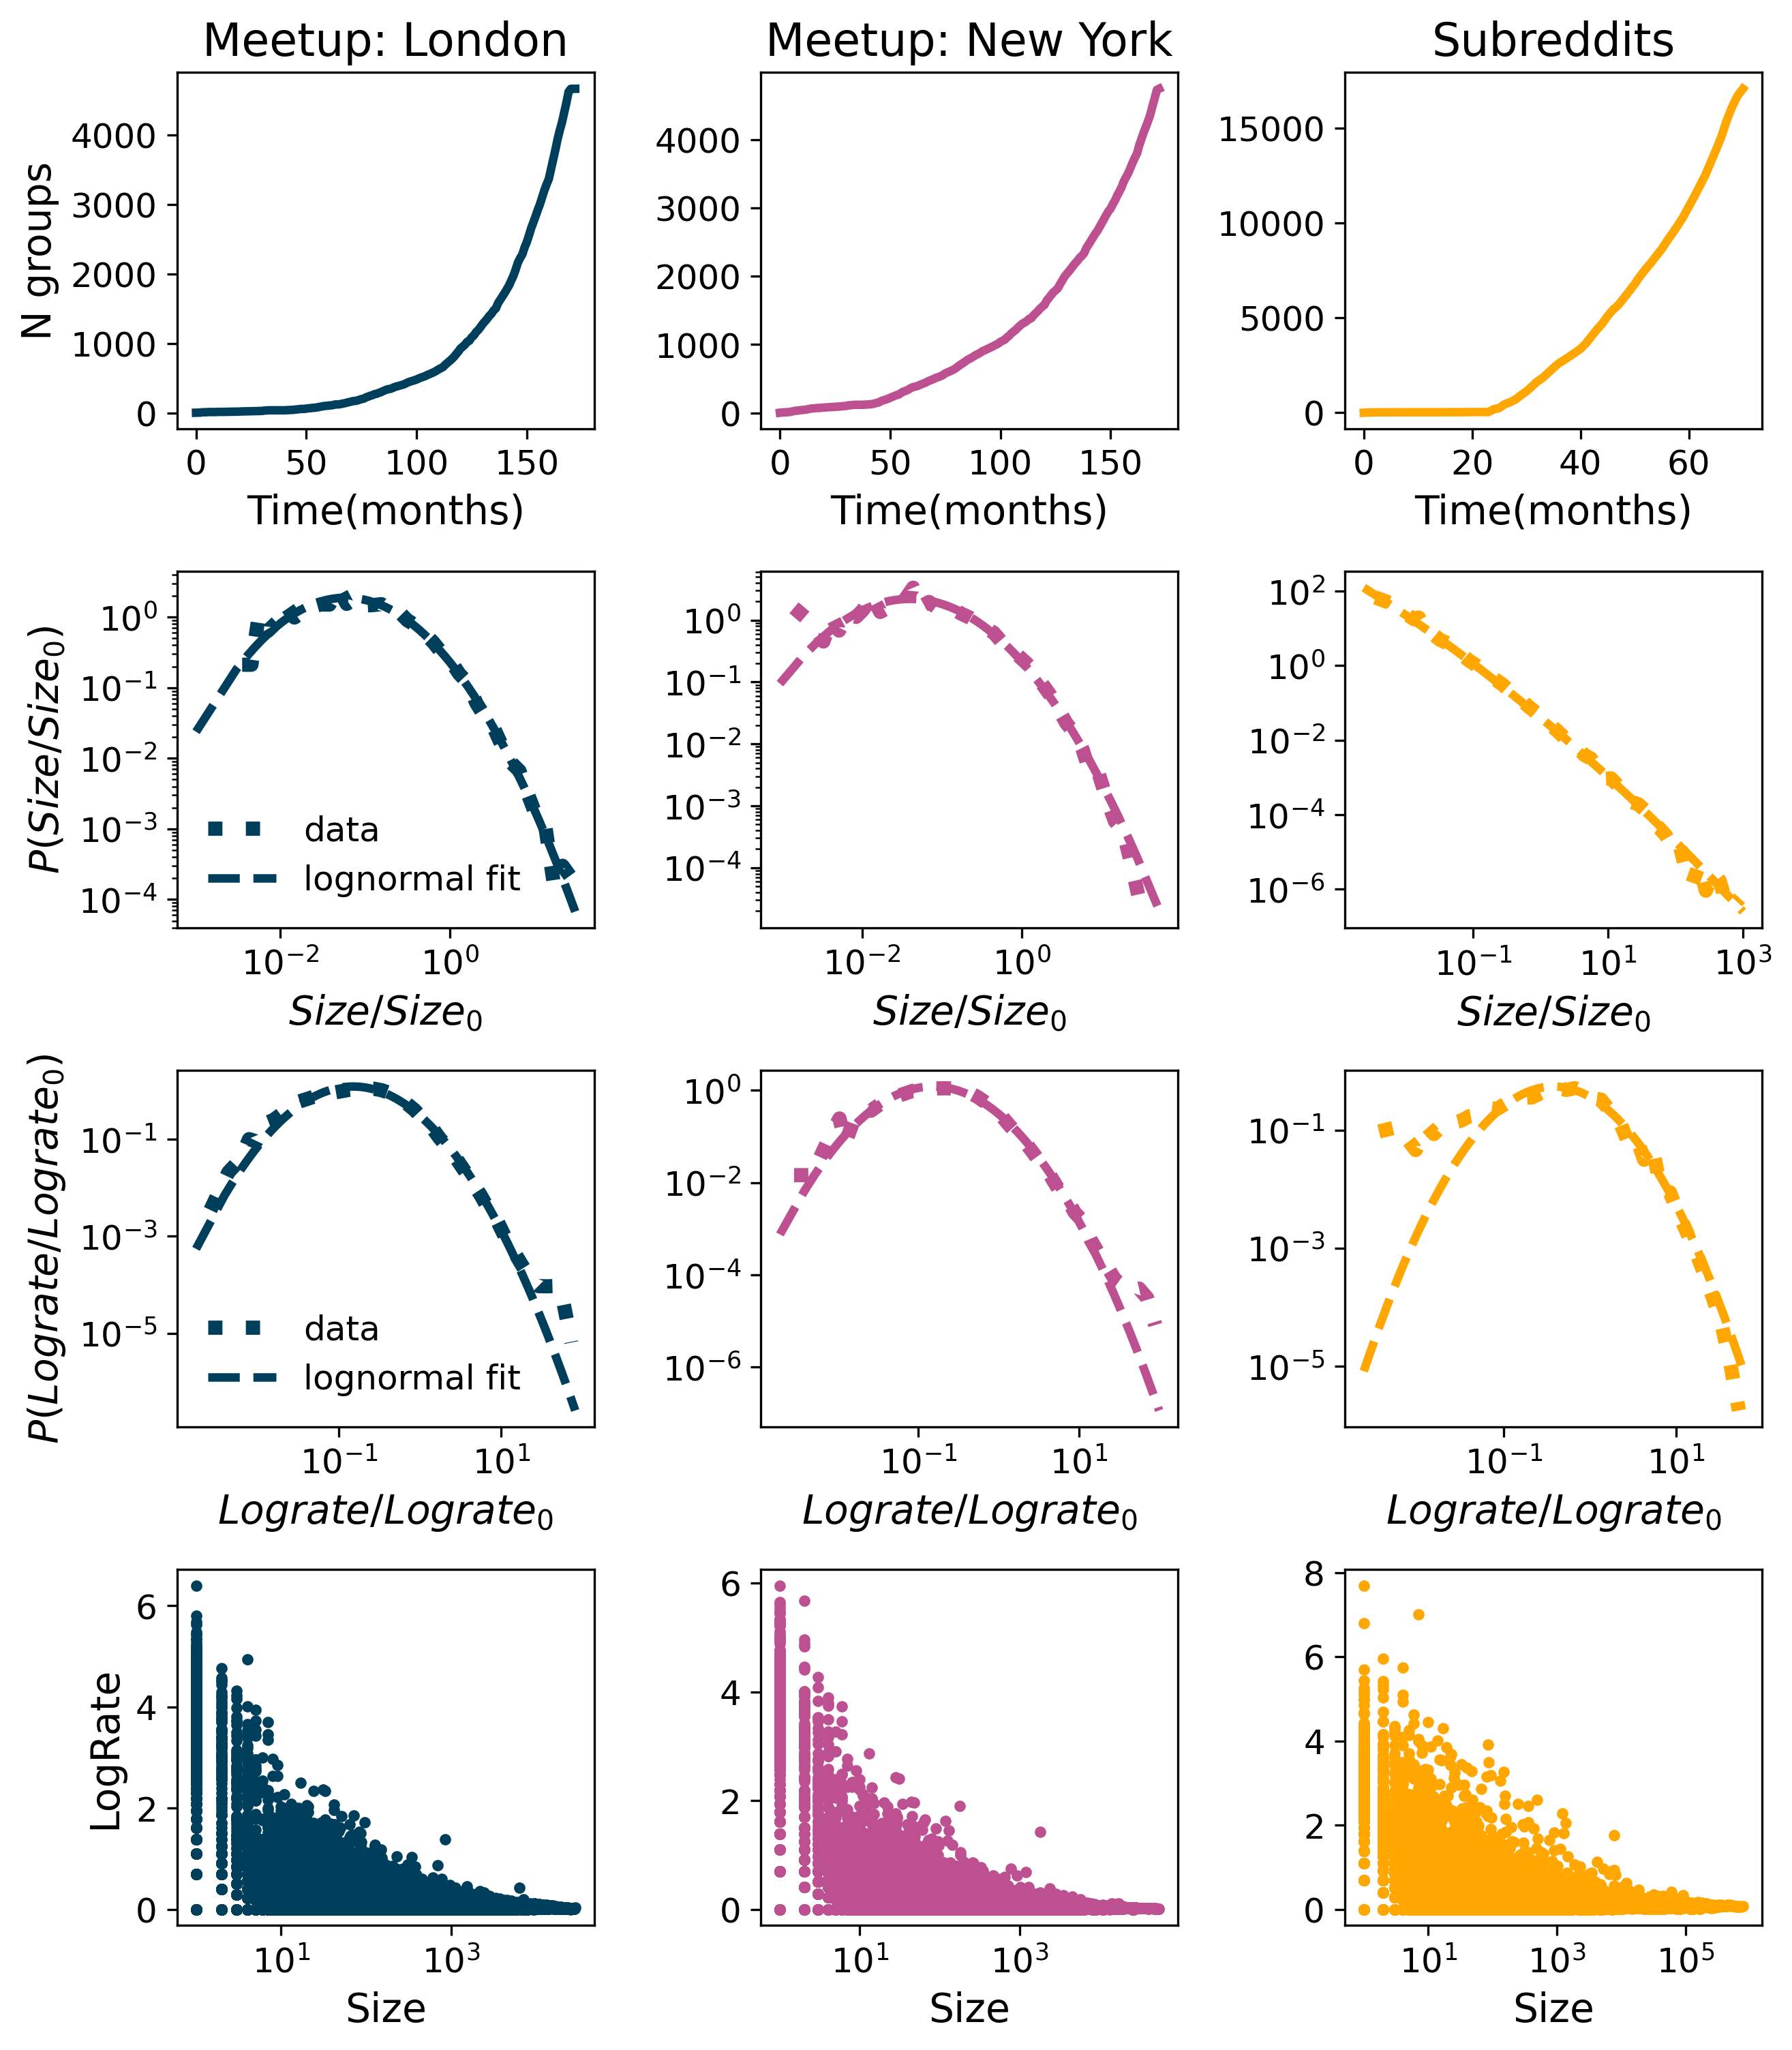
\includegraphics[width=0.8\linewidth]{Figures/figures/Fig2.png}
	\caption[Properties of Meetup and Subreddit groups]{The number of groups over time, normalized sizes distribution, normalized log-rates distribution and dependence of log-rates and group sizes for Meetup groups created in London from 08-2002 until 07-2017 that were active in 2017 and subreddits created in the period from 01-2006 to the  12-2011 that were active in 2017. }
	\label{fig:data1}
\end{figure}   

Even though Meetup and Reddit are different online platforms, we find some common properties of these systems; see figure \ref{fig:data1}. The number of groups and the number of new users grow exponentially. Still, subreddits are larger groups than Meetups. The distribution of groups sizes follows the log-normal distribution:
\begin{equation}
P(S)=\frac{1}{S\sigma\sqrt{2\pi}}exp(-\frac{(\ln(S)-\mu)^{2}}{2\sigma^{2}})
\label{eq:log}
\end{equation}
where $S$ is the group size and $\mu$, and $\sigma$ are parameters of the distribution.

The distributions for Meetup group sizes in London and New York follow similar log-normal distribution, with parameters $\mu= -0.93$, $\sigma = 1.38$ for London and $\mu=-0.99$ and $\sigma=1.49$ for New York. The group sizes distribution of Subreddits is a broad log-normal distribution that resembles the power law, it has parameters $\mu= -5.41$ and $\sigma = 3.07$.   Still, we used the log-likelihood ratio method and showed that log-normal distribution is better fit for these data then the power-law. In the Result section is given detailed analysis that support this findings.   

The simplest model that generates the lognormal distribution is multiplicative process \cite{mitzenmacher2004brief}. Gibrat used this model to explain the growth of firms. The main assumption of this model is that growth rates  $R = log\frac{S_t}{S_{t-\Delta t}}$ do not depend on the size $S$ and that they are uncorrelated. Further, this imply the lognormal distribution of the sizes, while the distribution of growth rates appears to be normal distribution,  \cite{mondani2014fat}, \cite{fu2005growth}. Figure \ref{fig:scale} shows distribution of the logrates, that follow lognormal distribution, contrary to the Gibrat law. Furthermore, logrates depend on the group size \ref{fig:scale}. For these reasons the Gibrat law can not explain the growth of online social groups. Similar conclusion are shown in recent studies about cities or growth of the internet \cite{frasco2014spatially, qian2014origin}.   

The growth of online social groups has universal behavior. It is independent on the size of the group. If we aggregate the groups created in the same year $y$, and each group size normalize with average size $<S^y>$, $s^{y}_{i}=S^{y}_{i}/<S^{y}>$ we will find that group sizes distributions for the same dataset and different years fall on the same line, figure \ref{fig:scale}. The same characteristics are observed for the distribution of the normalized logrates \ref{fig:scale}. The growth is universal in time, and the group sizes distribution do not change from year to year.

\begin{figure}[h]
	\centering
	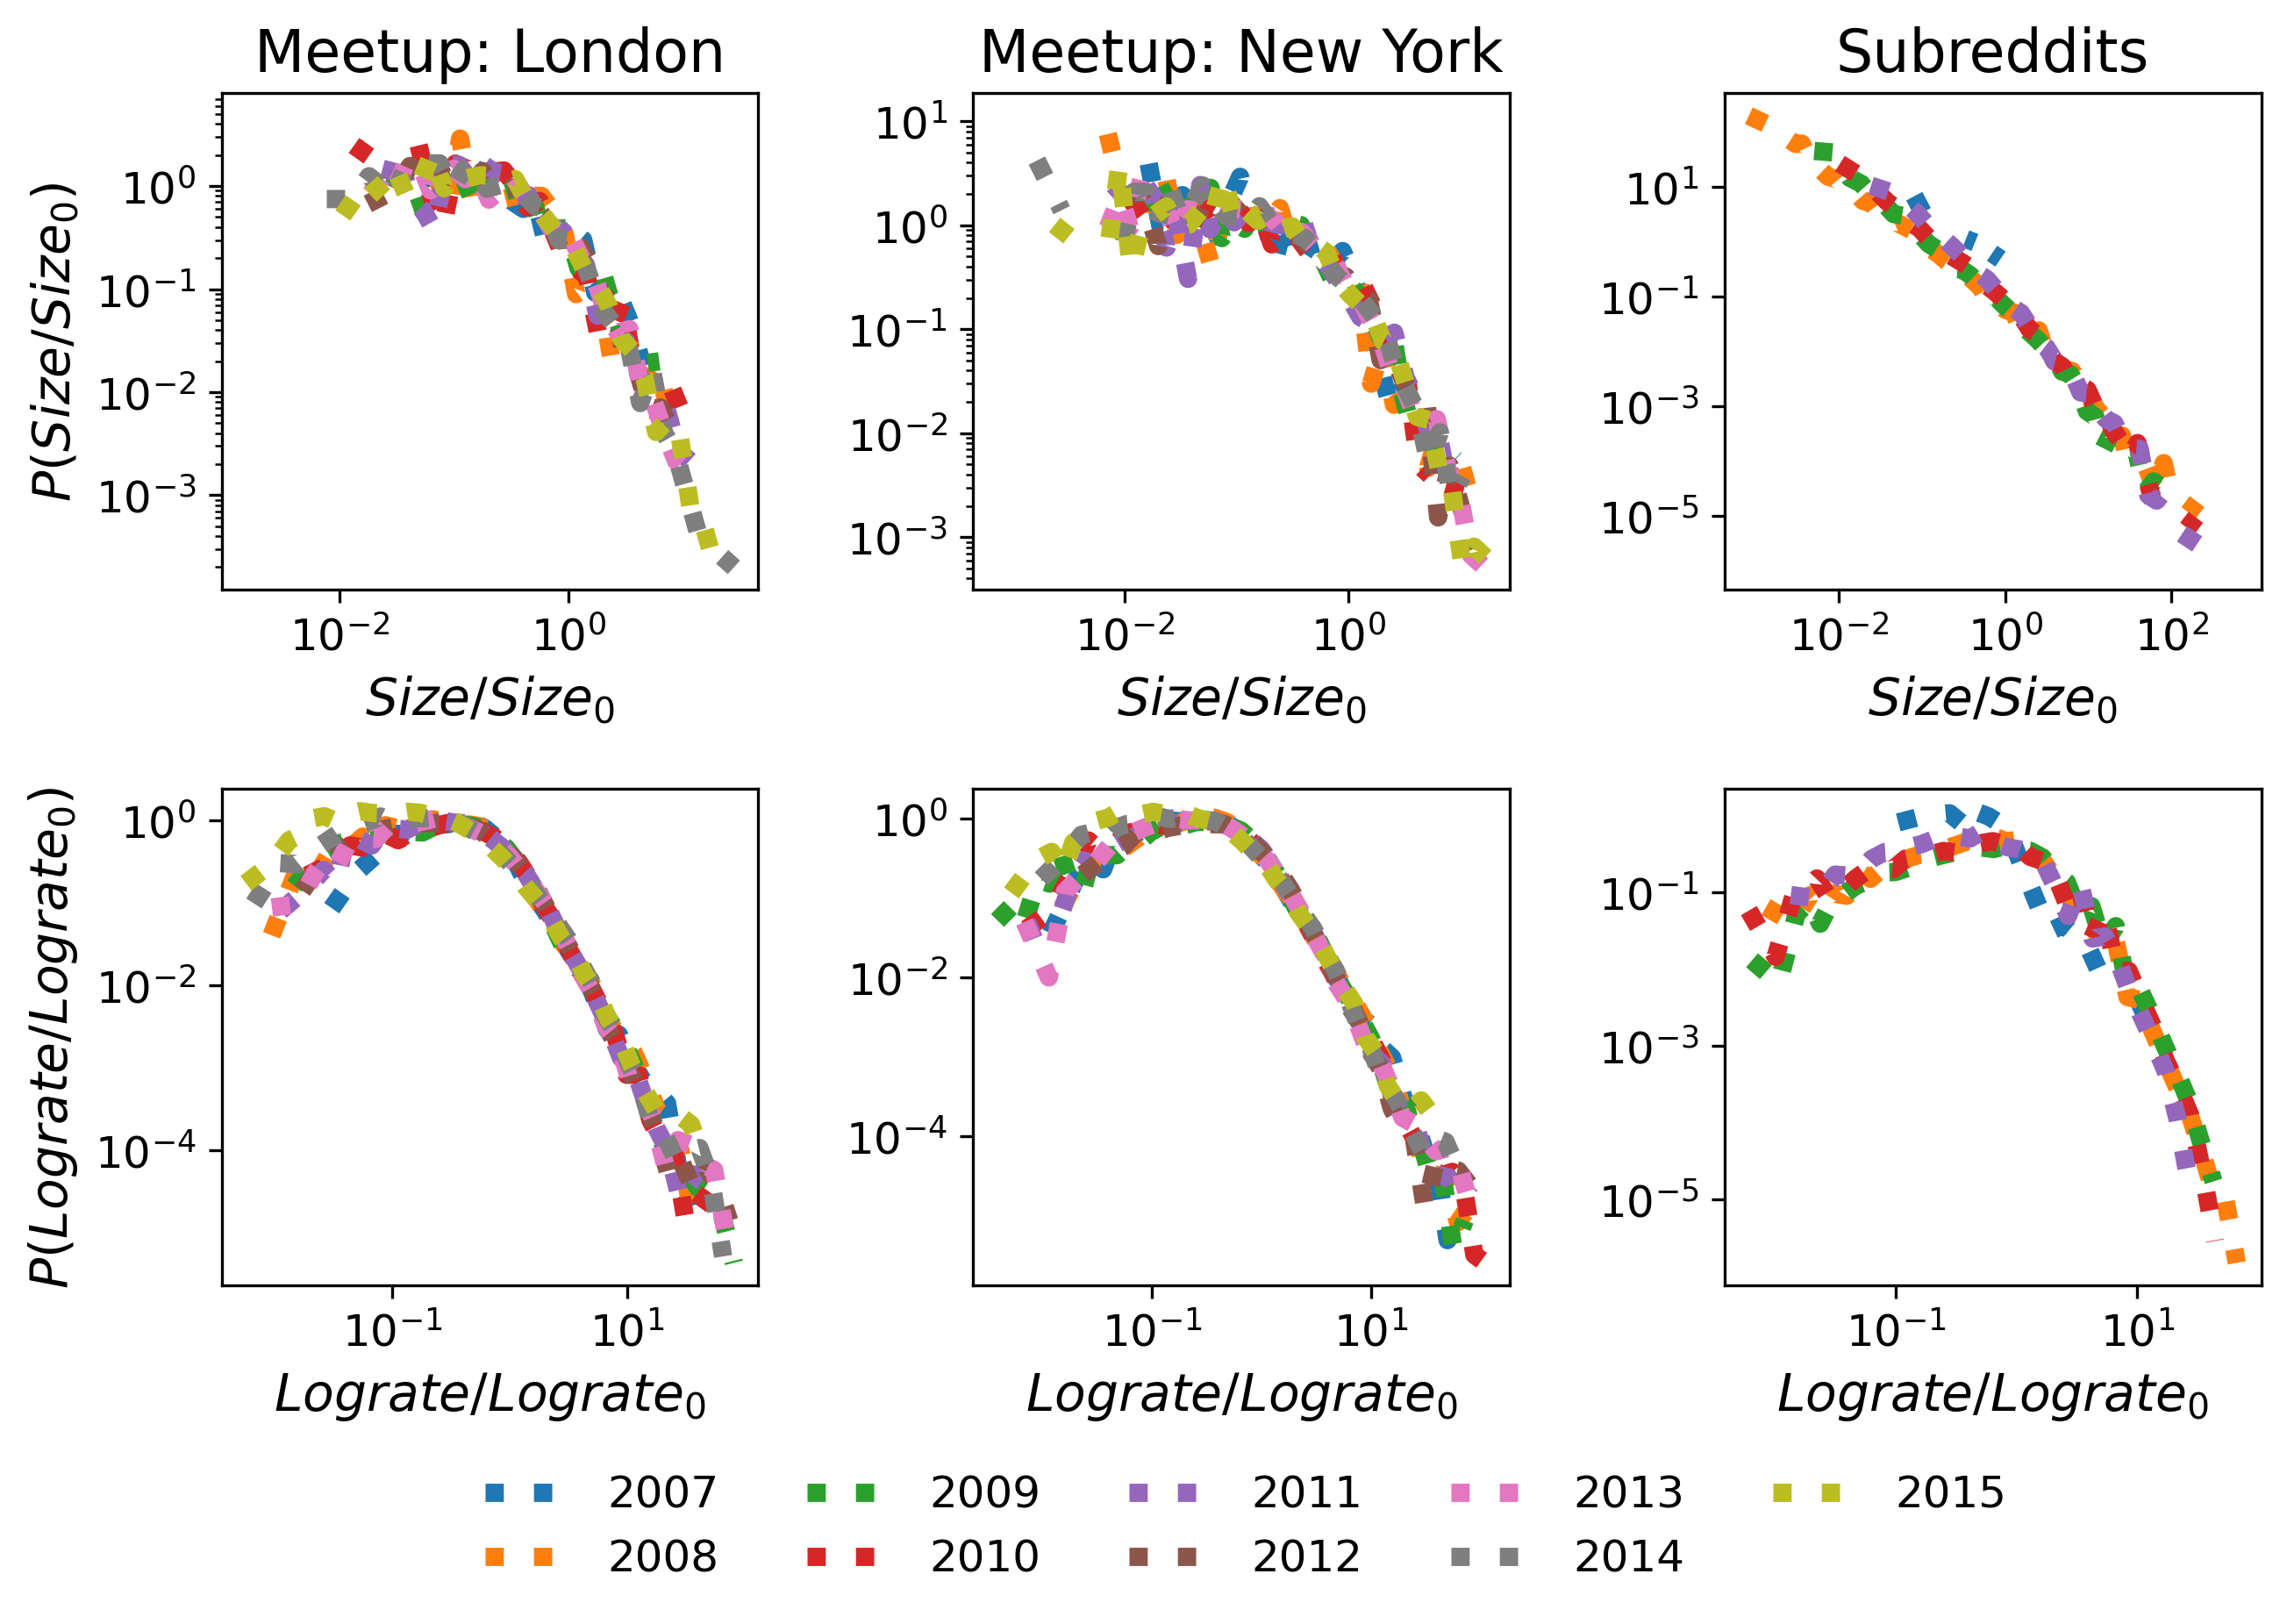
\includegraphics[width=0.8\linewidth]{Figures/figures/Fig1.png}
	\caption[Universality in the Meetup and Reddit groups]{The figure shows the groups' sizes distributions and log-rates distributions. Each distribution collects groups founded in the same year and is normalized with its mean value. The group sizes are at the end of 2017 for meetups and 2011 for subreddits.}
	\label{fig:scale}
\end{figure}

\section{The model}

Meetup and Reddit engage members in different activities. Still, there are some underlying processes same in both systems. Each member can create new groups and join existing ones. Both systems grow in the number of groups and users, and each user can belong to arbitrary number of groups. In the previous section, we identified the universal patterns in the growth of social groups, but it appears that the growth can not be modelled with Gibrat law. 

The complex network models allow us to simulate the growth of these systems considering all types of members' activities. We can identify how model parameters shape the growth process by varying linking rules.
Regarding the user's group choice, it was shown that social connections play an important role \cite{kairam2012life, zheleva2009co}. On the other hand, users can be driven by personal interests. Diffusion between groups could also be enhanced with rich-get-richer phenomena, where users tend to join larger groups. With a complex network model, we can easily incorporate the nonlinear growth in the number of users and groups, as it is an important parameter that shapes the structure and dynamics of the complex network \cite{mitrovic2011quantitative, dankulov2015dynamics, vranic2021growth}.

The evolution of the social groups has been studied using the co-evolution model in the reference  \cite{zheleva2009co}. This model consists of two evolving networks: the bipartite network, which stores connections between users and groups and the affiliation network of social connections. At each time step, active users create new connections in the affiliation network; i.e. they make new friends. They also join existing groups or create new ones, which updates the bipartite network. The group selection can be random with probability proportional to the group size; otherwise, the group is selected through social contacts. Using this model, authors have reproduced the power-law group size distribution found in several communities, such as Flickr or LiveJournal. The empirical analysis of Meetup and Reddit groups showed that group size distribution could be log-normal, meaning that some different mechanisms control the growth of the groups.

We propose a model that is based on the co-evolution model. The main difference between those two models is how model parameters are defined. First of all, in the co-evolution model user becomes inactive after period $t_a$, which is drawn from an exponential distribution with the rate $\lambda$, while in our model probability that the user is active is constant, and the same for each user. The second difference is how groups are chosen. While in the co-evolution model probability that the user selects a group through social linking depends on the friend's degree, we give preference to groups where a user has a larger number of social contacts. We also modified the rules for random linking, so users choose a group with uniform probability.

\subsection{Groups growth model}

The representation of the model is given in figure \ref{fig:schema}. The model consists of two networks:
\begin{itemize}
	\item bipartite network $\mathcal{B}(V_{U}, V_{G}, E_{UG})$, where $V_U$ is set of users, $V_G$ set of groups and $E_{UG}$ set of links between users and groups, where link $e(u,g)$ indicates that user $u$ is member of group $g$.
	\item social network $\mathcal{G}(V_{U},E_{UU})$ describes the social connections $e(u, v)$ between users $u$ and $v$, and  $V(U)$ is set of users same as in bipartite network. 
\end{itemize}

The bipartite and social networks evolve. At each step, new users $N_U(t)$ are added to the network. It is how the set of users $V_U$ in the bipartite and social network can grow. At arrival, each new member connects to a randomly selected user in the social network $G$. This allows new members to choose a group based on social contacts \cite{kairam2012life}. The activity of old members is a stochastic process; old members are activated with probability $p_a$. The set of active users $\mathcal{A}_{U}$ has new members $N_U(t)$ and old members who decided to be active in that time step.

The active users can create a new group with probability $p_g$. By this, group node $g$ is added to the set of group nodes $V_G$ in bipartite network $B$. If an active user does not create a new group, it will join the existing one with probability $1-p_g$, see lower panel on figure \ref{fig:schema}. When the user creates a new group or joins an existing one, the link $e(u,g)$ is made in the bipartite network $B$.

\begin{figure}[h]
	\centering
	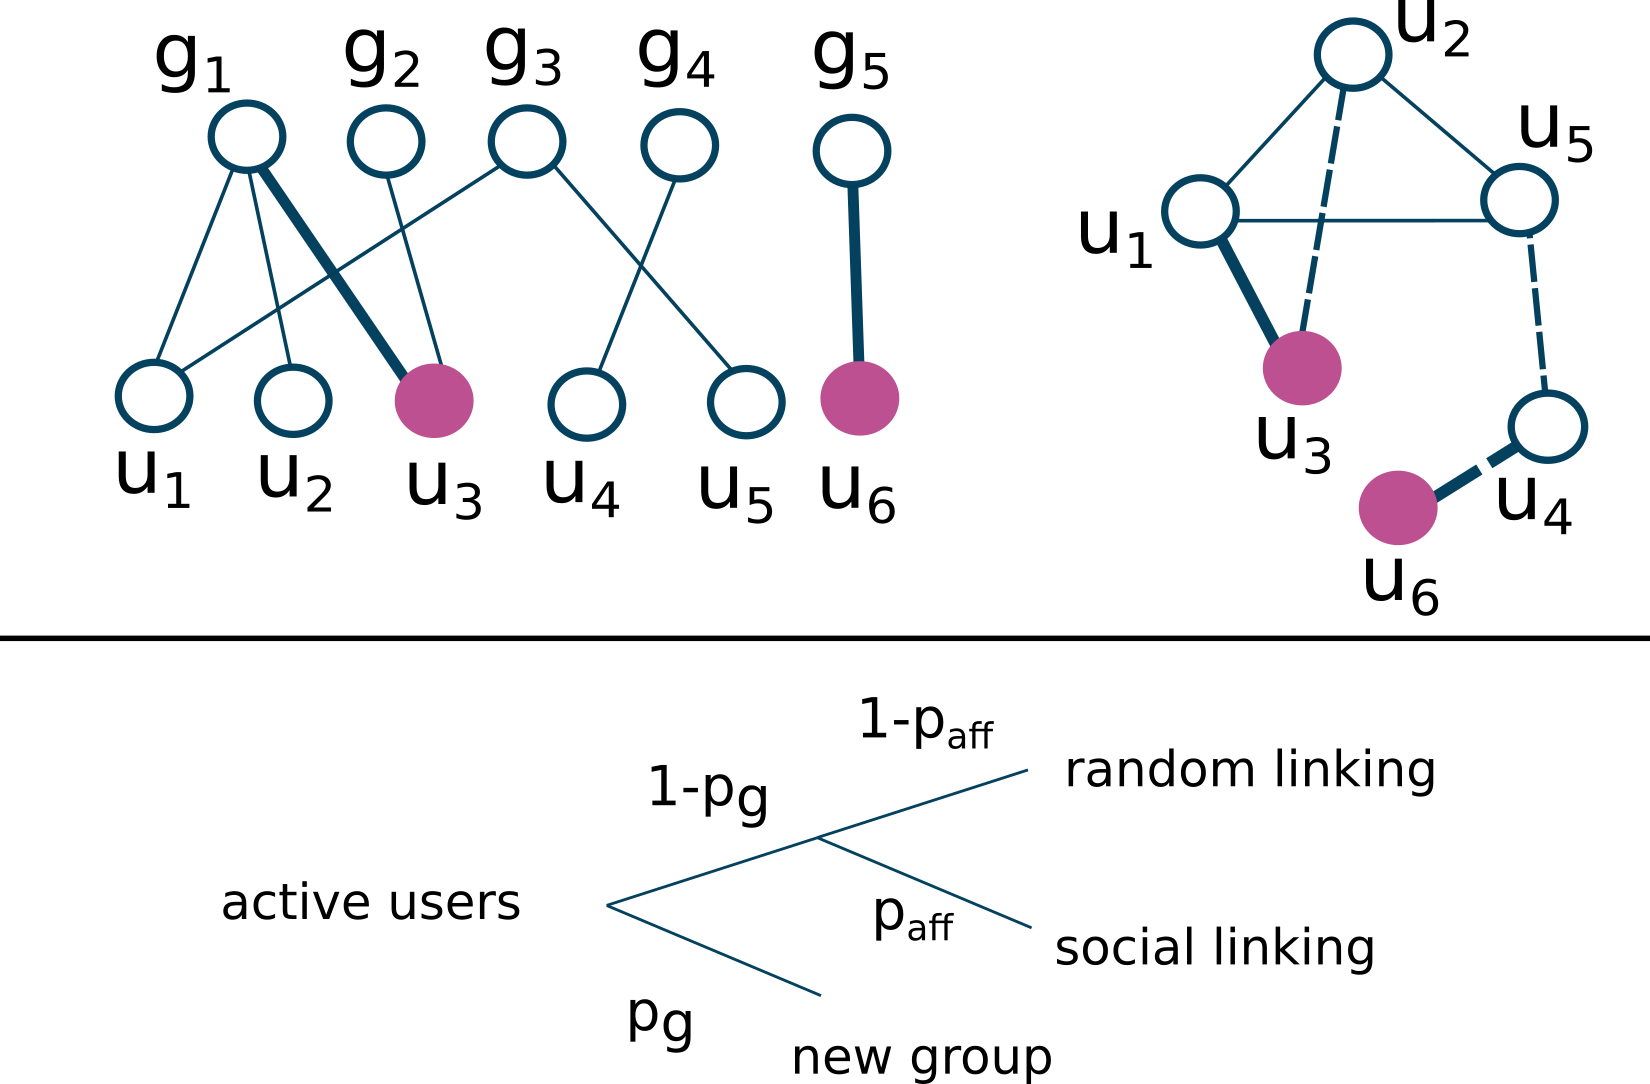
\includegraphics[scale=0.5]{Figures/figures/test.png}
	\caption[Bipartite groups growth model]{The top panel shows bipartite (member-group) and social (member-member) network. Filled nodes are active members, while thick lines are new links in this time step. In the social network dashed lines show that members are friends but still do not share same groups. The lower panel shows model schema, where $p_g$ is probability that user create new group, while $p_{aff}$ is probability that group choice depends on the social connections. \textbf{Example:} member $u_6$ is a new member. First it will make random link  with node $u_4$, and then with probability $p_g$ makes new group $g_5$. With probability $p_a$ member $u_3$ is active, while others stay inactive for this time step. Member $u_3$ will with probability $1-p_g$ choose to join one of old groups and with probability $p_{aff}$ linking is chosen to be social. As its friend $u_2$ is member of group $g_1$, member $u_3$ will also join group $g_1$. Joining group $g_1$, member $u_3$ will make more social connections, in this case it is member $u_1$.}
	\label{fig:schema}
\end{figure}

When joining existing groups, users may be influenced by social connections. This linking happens with probability $p_{aff}$. The second case is that the user chooses a random group with probability $1-p_{aff}$. 

Social linking depends on the properties of a bipartite and social network. The networks can be represented with matrices $B$ and $A$, so if a link between two nodes exists, they have element $1$. The neighbourhood of user $u$, $\mathcal{N}_{u}$ in a bipartite network is a set of groups in which the user is a member. Similarly, we define the neighbourhood of group $g$ as $N_g$, as a set of users who belong to the group. From there, we can define the probability $ P_{ug}$ that the user $u$ will choose group $g$. This probability is proportional to the number of social contacts that the user has in the group. 

\begin{equation}
P_{ug}=\sum_{u_{1}\in \mathcal{N}_{g}} A_{uu_{1}} 
\label{eq1}
\end{equation}

After selecting group $g$, user $u$ is introduced to new members in the group and can make new social contacts. In the simplest case, we could assume that all members belonging to a group are connected. However, previous research on this subject \cite{ smiljanic2017associative, backstrom2006group, zheleva2009co} has shown that the existing social connections of members in a social group are only a subset of all possible connections. We select $X$ random members $u_i$ from group $g$ and make new connections in social network $e(u, u_i)$. 

The model parameters $p_a$ and $p_g$ are important for controlling the number of users and groups. With larger parameter values $p_a$, more users become active, and the number of links in bipartite and social networks grows faster. Parameter $p_g$ controls the rate at which new groups are created. For example, if $p_g=0$, users will not create new groups. Also, if $p_g=1$, users will only create new groups, and the resulting network will consist of star-like subgraphs. In real systems we do not expect extreme values for probabilities $p_a$ and $p_g$. First, not all members are constantly active, and we do not find a burst in the creation of the groups. From real data, we notice that there is always a higher number of users than groups in social systems. The parameter $p_{aff}$ how users choose groups, and with higher $p_{aff}$ social connections become more important. 

\subsection{Dependence of the group size distribution on model parameters}

Before applying the group growth model on Meetup and Reddit, we consider the system where at each time step, a constant number of users is added $N(t)=30$. We also fix the probability that user is active to $p_a=0.1$, so we can in more details explore the influence of parameters $p_g$ and $p_{aff}$. We plot the group size distribution after $60$ steps of simulation. The values of $p_g$ and the $p_a$ influence the number of groups, their maximum size, and the shape of group size distribution. With probability $p_g=0.1$, users create large number of groups, over $10^4$, while with $p_g=0.5$ they are on the order of magnitude $10^5$. 

Figure \ref{fig:n30} show the obtained group size distributions with power-law and log-normal fits. For lower value of parameter $p_g=0.1$ and $p_{aff}=0$, users join randomly chosen groups. Group size distributions are approximated with log-normal. When the affiliation parameter is larger, $p_{aff}=0.5$, the log-normal distribution becomes broader, and so on, we find the larger maximum group size. 

If we increase the parameter $p_g=0.5$, every second active user will create a group. At this group creation rate, the group size distribution deviates from log-normal, but it is not explained with power-law either, right column on figure \ref{fig:n30}.

\begin{figure}[!ht]
	\centering
	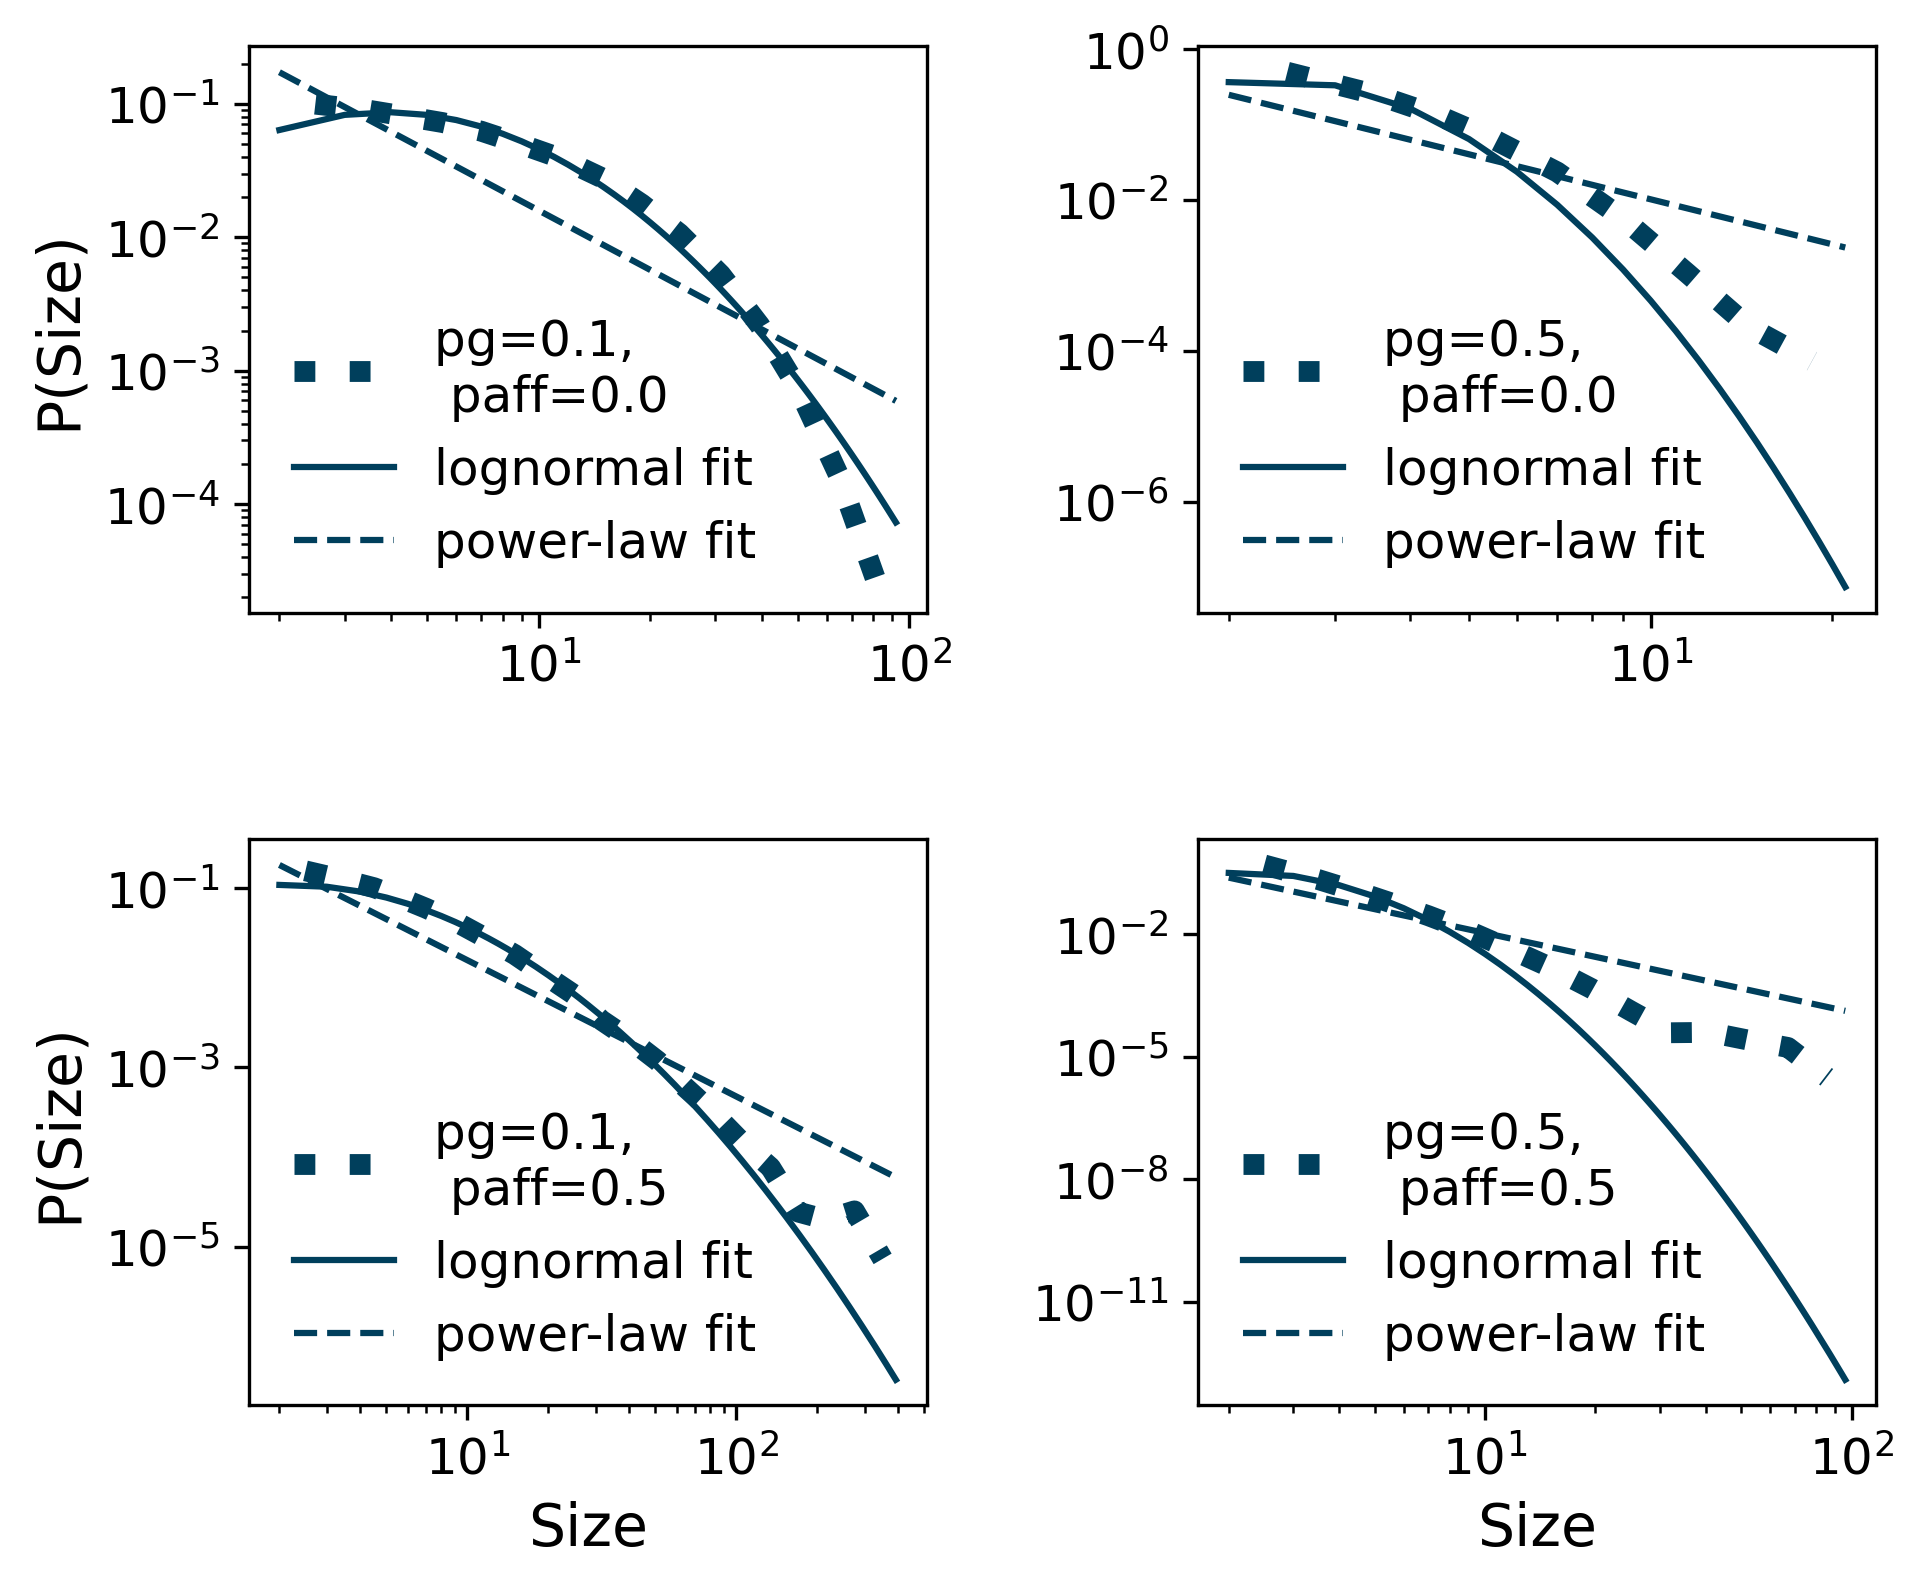
\includegraphics[width=0.7\linewidth]{Figures/figures/Fig5_a.png}
	%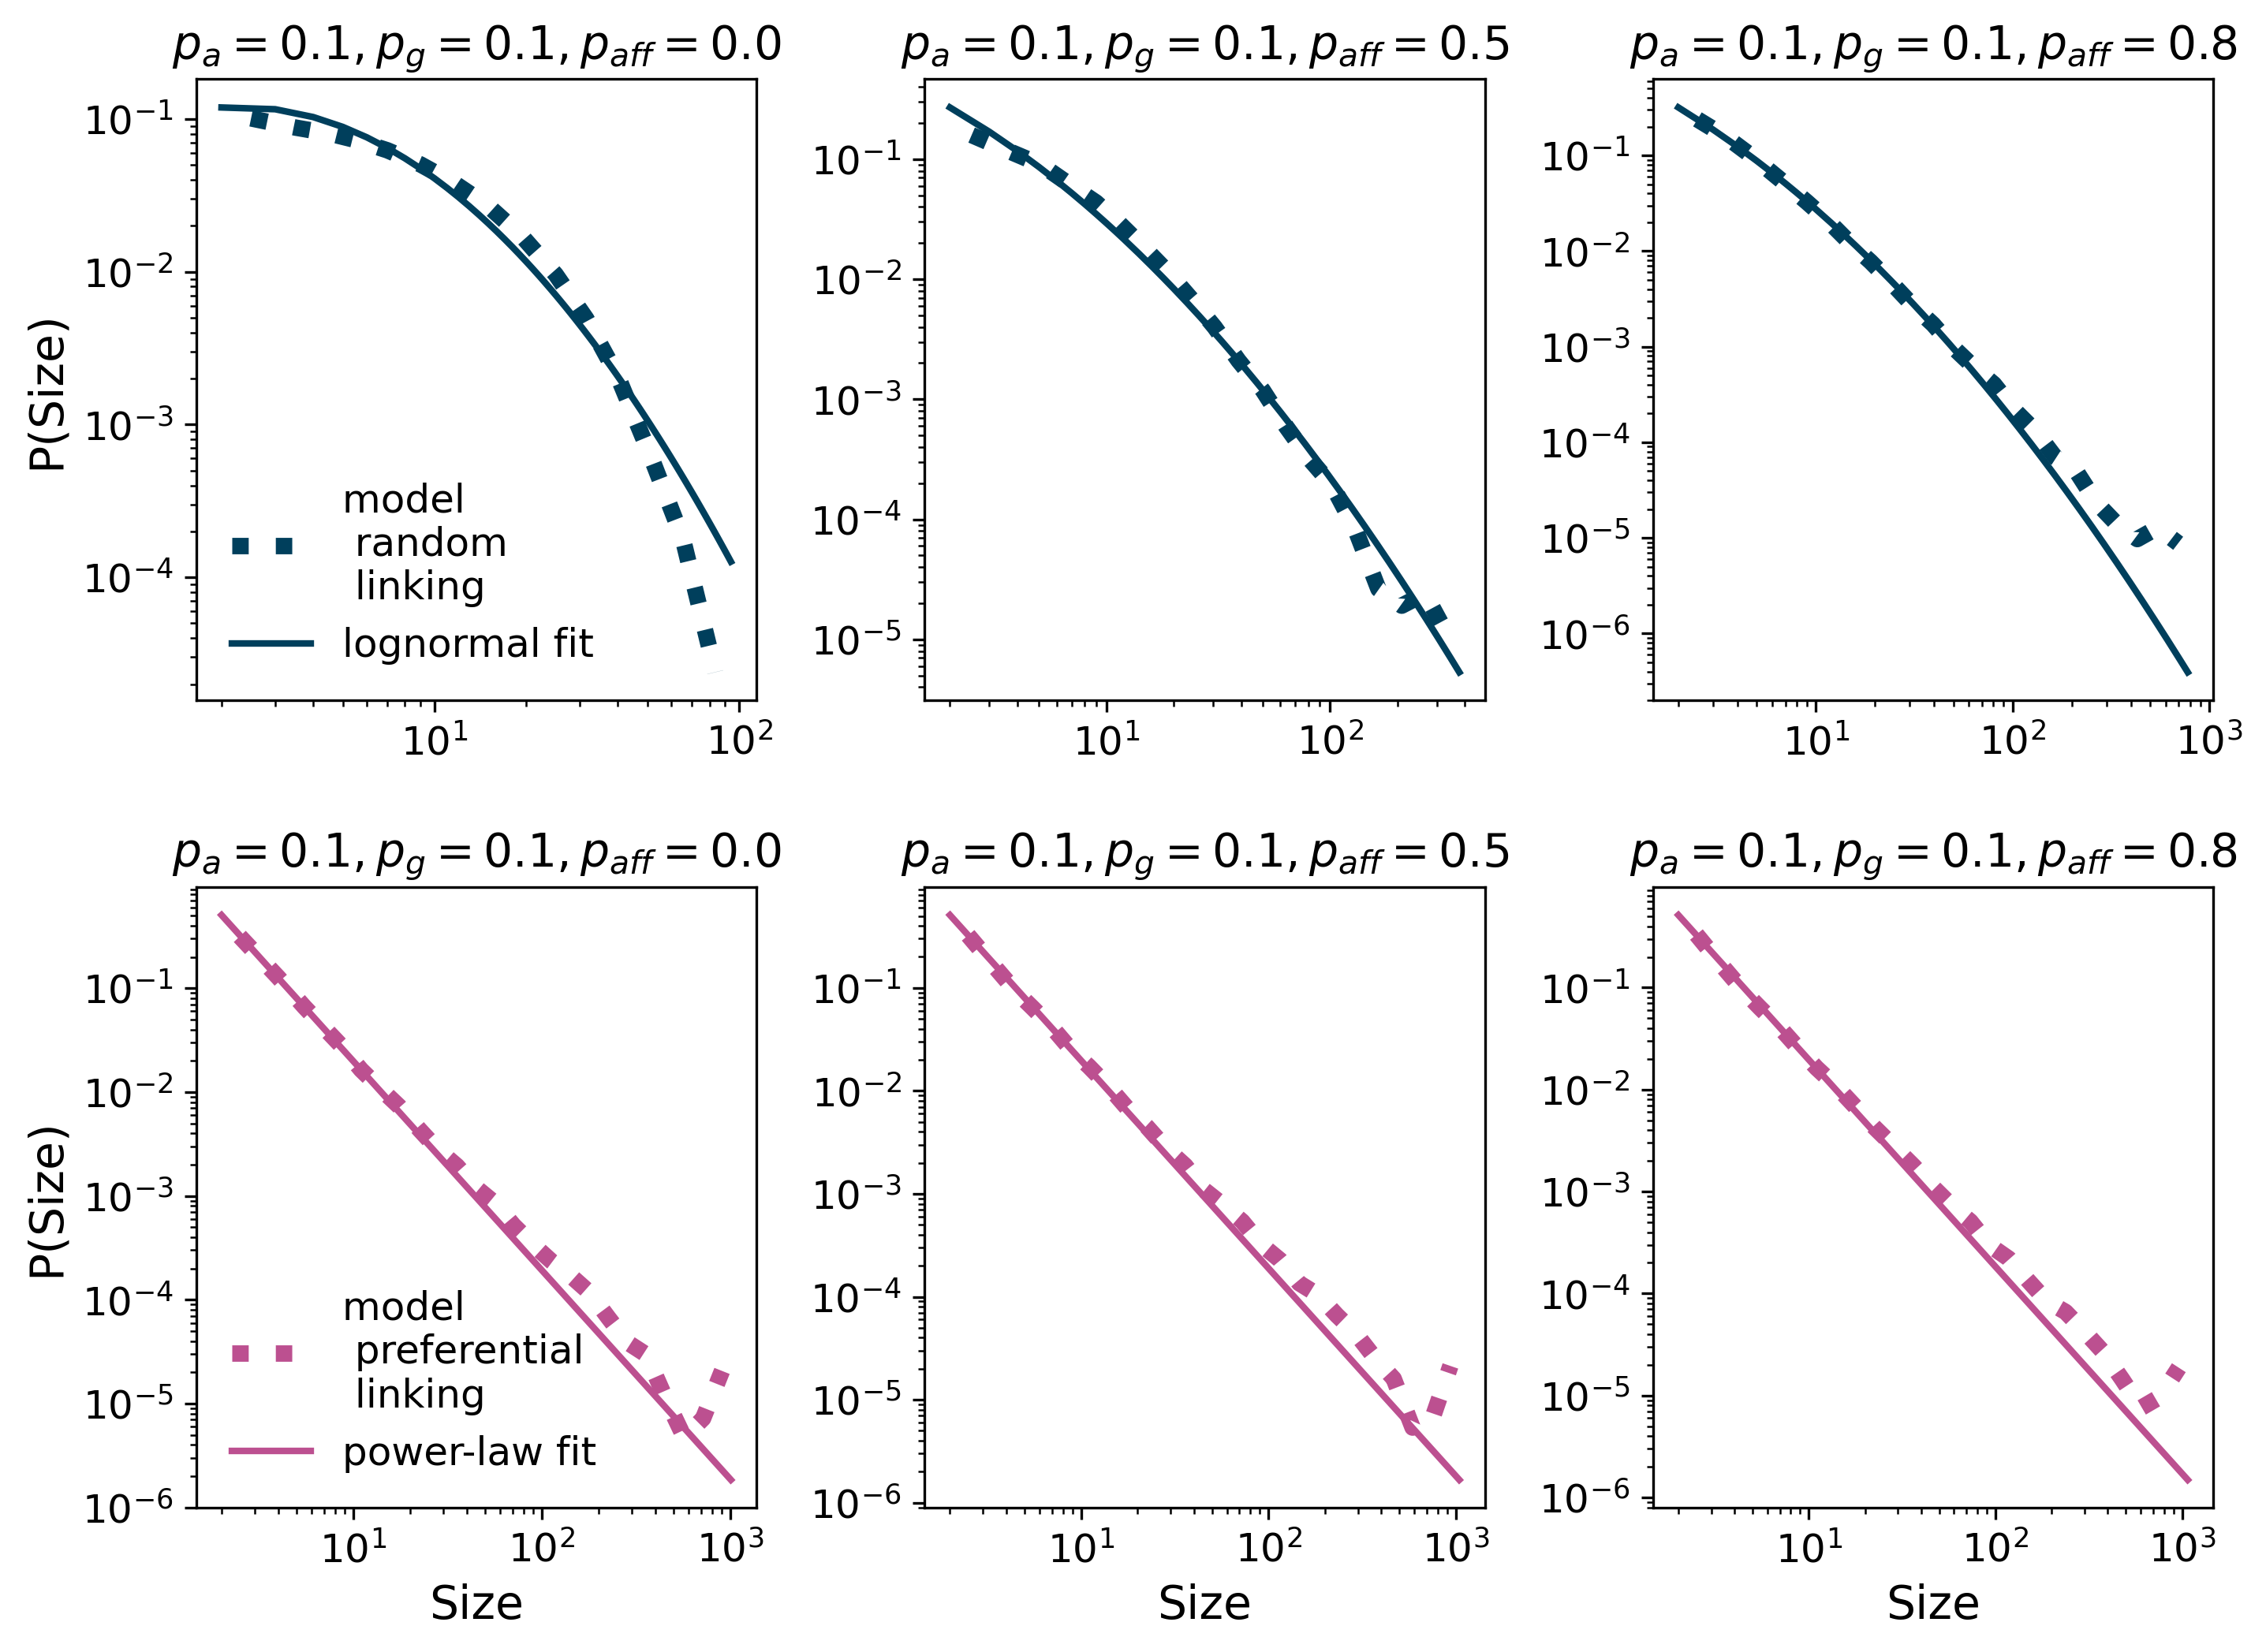
\includegraphics[width=0.8\linewidth]{figures/model_N30.png}
	\caption[Group size distribution for different model parameters]{The distribution of sizes for different values of $p_{g}$ and $p_{aff}$ and constant $p_{a}$ and growth of the system. The combination of the values of parameters of $p_{g}$ and $p_{aff}$ determine the shape and the width of the distribution of group sizes. }
	\label{fig:n30}
\end{figure}

Finally, we compare how group size distribution depends on different rules in random linking. In our model, the probability that the user chooses a random group is uniform. In contrast, in the co-evolution model \cite{zheleva2009co}, probability depends on the group size, as in the preferential attachment model. Instead of random linking, if we incorporate preferential linking, so users with probability $1-p_{aff}$ tend to choose larger groups, group size distribution changes significantly. Similar to the co-evolution model, we find the power-law distribution. Figure \ref{fig:model_comp} shows the results from a model where we add a constant number of new users at each time step. The probabilities $p_a$ and $p_g$ are fixed, and affiliation parameter takes values $0$, $0.5$ and $0.8$. If we consider random linking , top panel on figure \ref{fig:model_comp}, the distribution becomes broader with larger $p_{aff}$. On the other hand, with preferential linking, group size distribution is a power-law and the $p_{aff}$ parameter does not have a large impact on the distribution shape.    

\begin{figure}[h]
	\centering
	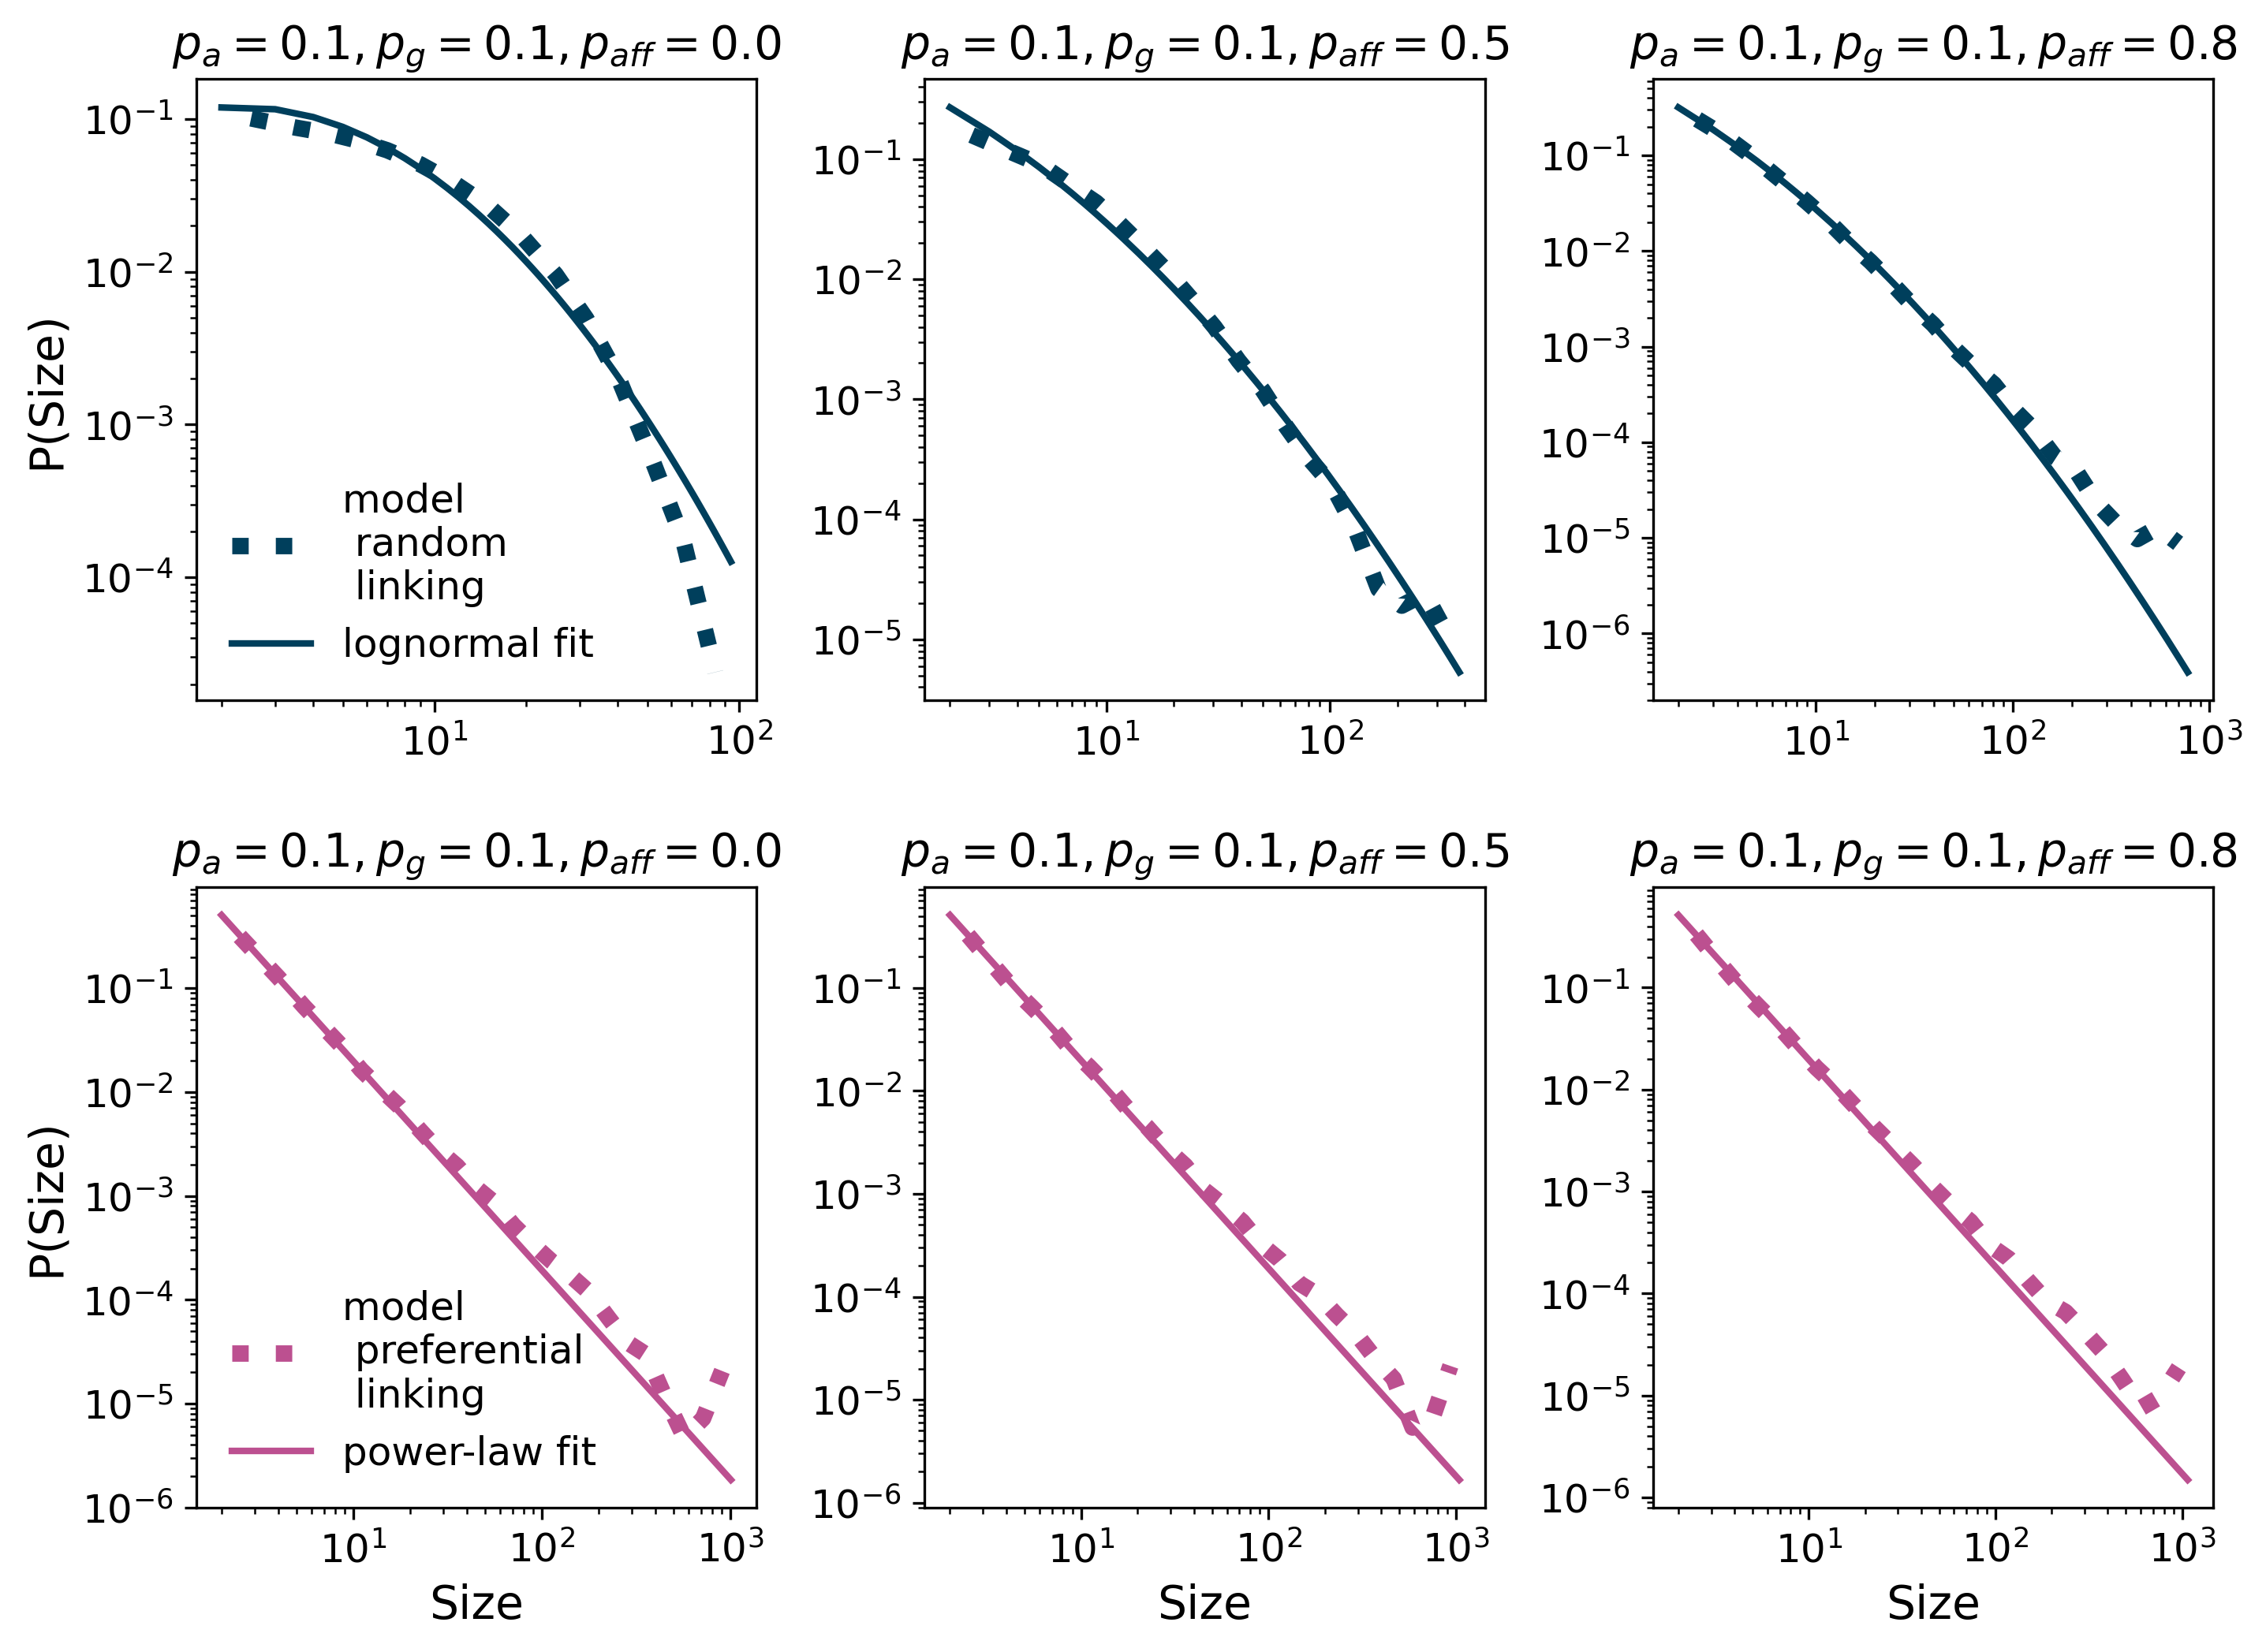
\includegraphics[width=0.7\linewidth]{figures/model_N30.png}
	\caption[Comparison between preferential and random linking in groups growth model.]{Groups sizes distributions for groups model, where at each time step the constant number of users arrive, $N=30$ and old users are active with probability $p_a=0.1$. Active users make new groups with probability $p_g=0.1$, while we vary affiliation parameter $p_{aff}$. With probability, $1-p_{aff}$, users choose a group randomly. The group sizes distribution (top row) is described with a log-normal distribution. With higher affiliation parameter, $p_{aff}$, distribution has larger width. The bottom row presents the case where with probability $1-p_{aff}$ users have a preference toward larger groups. For all values of parameter $p_{aff}$, we find the power-law group sizes distribution.}
	\label{fig:model_comp}
\end{figure}


%How members are distributed in these groups depends on the value of parameter $p_{aff}$. When $p_{aff}=0$, social connections are irrelevant for the choice of the group and members choose groups at random. The obtained distribution slightly deviates from log-normal, especially for large group sizes. In this case large groups sizes become more probable than in the case of log-normal distribution. The non zero value of parameter $p_{aff}$ means that the choice of group becomes dependent on social connections. 

%When member chooses a group according to her social connections, larger groups have higher probability to be affiliated with social connections of active members, and thus this choice resembles preferential attachment. For these reasons, the obtained size distribution has more broad tail than log-normal distribution, and begins to resemble power-law distribution.

%The differences between our and co-evolution model, described in previous sections, at first glance may appear small. However, they lead to huge differences in the distribution of the size of social groups. The distribution of group sizes in co-evolution model is a power-law. Our model adds flexibility to produce groups with log-normal size distribution. This expands classes of social systems that can be modeled. 
%Our model is more flexible and can produce groups with log-normal size distribution that better describes diverse social systems, including, ones described in the Section \ref{sec:emp}.\\

\section{Results}

The social systems do not grow at constant rate. In Ref. \cite{vranic2021growth} authors have shown that features of growth signal influence the  structure of social networks. For these reasons we use the real growth signal from Meetup groups located in London and New York, and Reddit community to simulate the growth of the social groups in these systems. Figure \ref{fig:fig5} top panel shows the time series of the number of new members that join each of the three systems each month. All three systems have relatively low growth at the beginning, and than the growth accelerates as the system becomes more popular.

We also use empirical data to estimate $p_{a}$, $p_{g}$ and $p_{aff}$. Probabilities that old members are active $p_a$ and that new groups are created $p_g$ can be approximated directly from the data. Activity parameter $p_{a}$ is the ratio between the number of old members that were active in month $t$ and the total number of members in the system at time $t$. Figure \ref{fig:fig5} middle row shows the variation of parameter $p_{a}$ during the considered time interval for each system. The values of this parameter fluctuates between $0$ and $0.2$ for London and New York based Meetup groups, while its value is between $0$ and $0.15$ for Reddit. To simplify our simulations we assume that $p_{a}$ is constant in time, and estimate its value as its median value during the $170$ months for Meetup systems, and $80$ months of Reddit system. For Meetup groups based in London and New York $p_{a}=0.05$, while Reddit members are more active on average and $p_{a}=0.11$ for this system.

Figure \ref{fig:fig5} bottom row shows the evolution of parameter $p_{g}$ for the three considered systems. The $p_{g}$ in month $t$ is estimated as the ratio between the groups created in month $t$ $Ng_{new}(t)$ and the total number of groups that month $Ng_{new}(t)+Ng_{old}(t)$, i.e., $p_{g}(t)=\frac{Ng_{new}(t)}{N_{new}(t)+N_{old}(t)}$. We see from Fig. \ref{fig:fig5} that $p_{g}(t)$ has relatively high values at the beginning of the system's existence. This is not surprising. At the beginning these systems have relatively small number of groups and often cannot meet the needs for content of all their members. As the time passes, the number of groups grows, as well as content offerings within the system, and members no longer have a high need to create new groups. Figure \ref{fig:fig5} shows that $p_{g}$ fluctuates less after the first few months, and thus we again assume that $p_{g}$ is constant in time and set its value to median value during 170 months for Meetup and 80 months for Reddit. For all three systems $p_{g}$ has the value of $0.003$.

\begin{figure}[h]
	\centering
	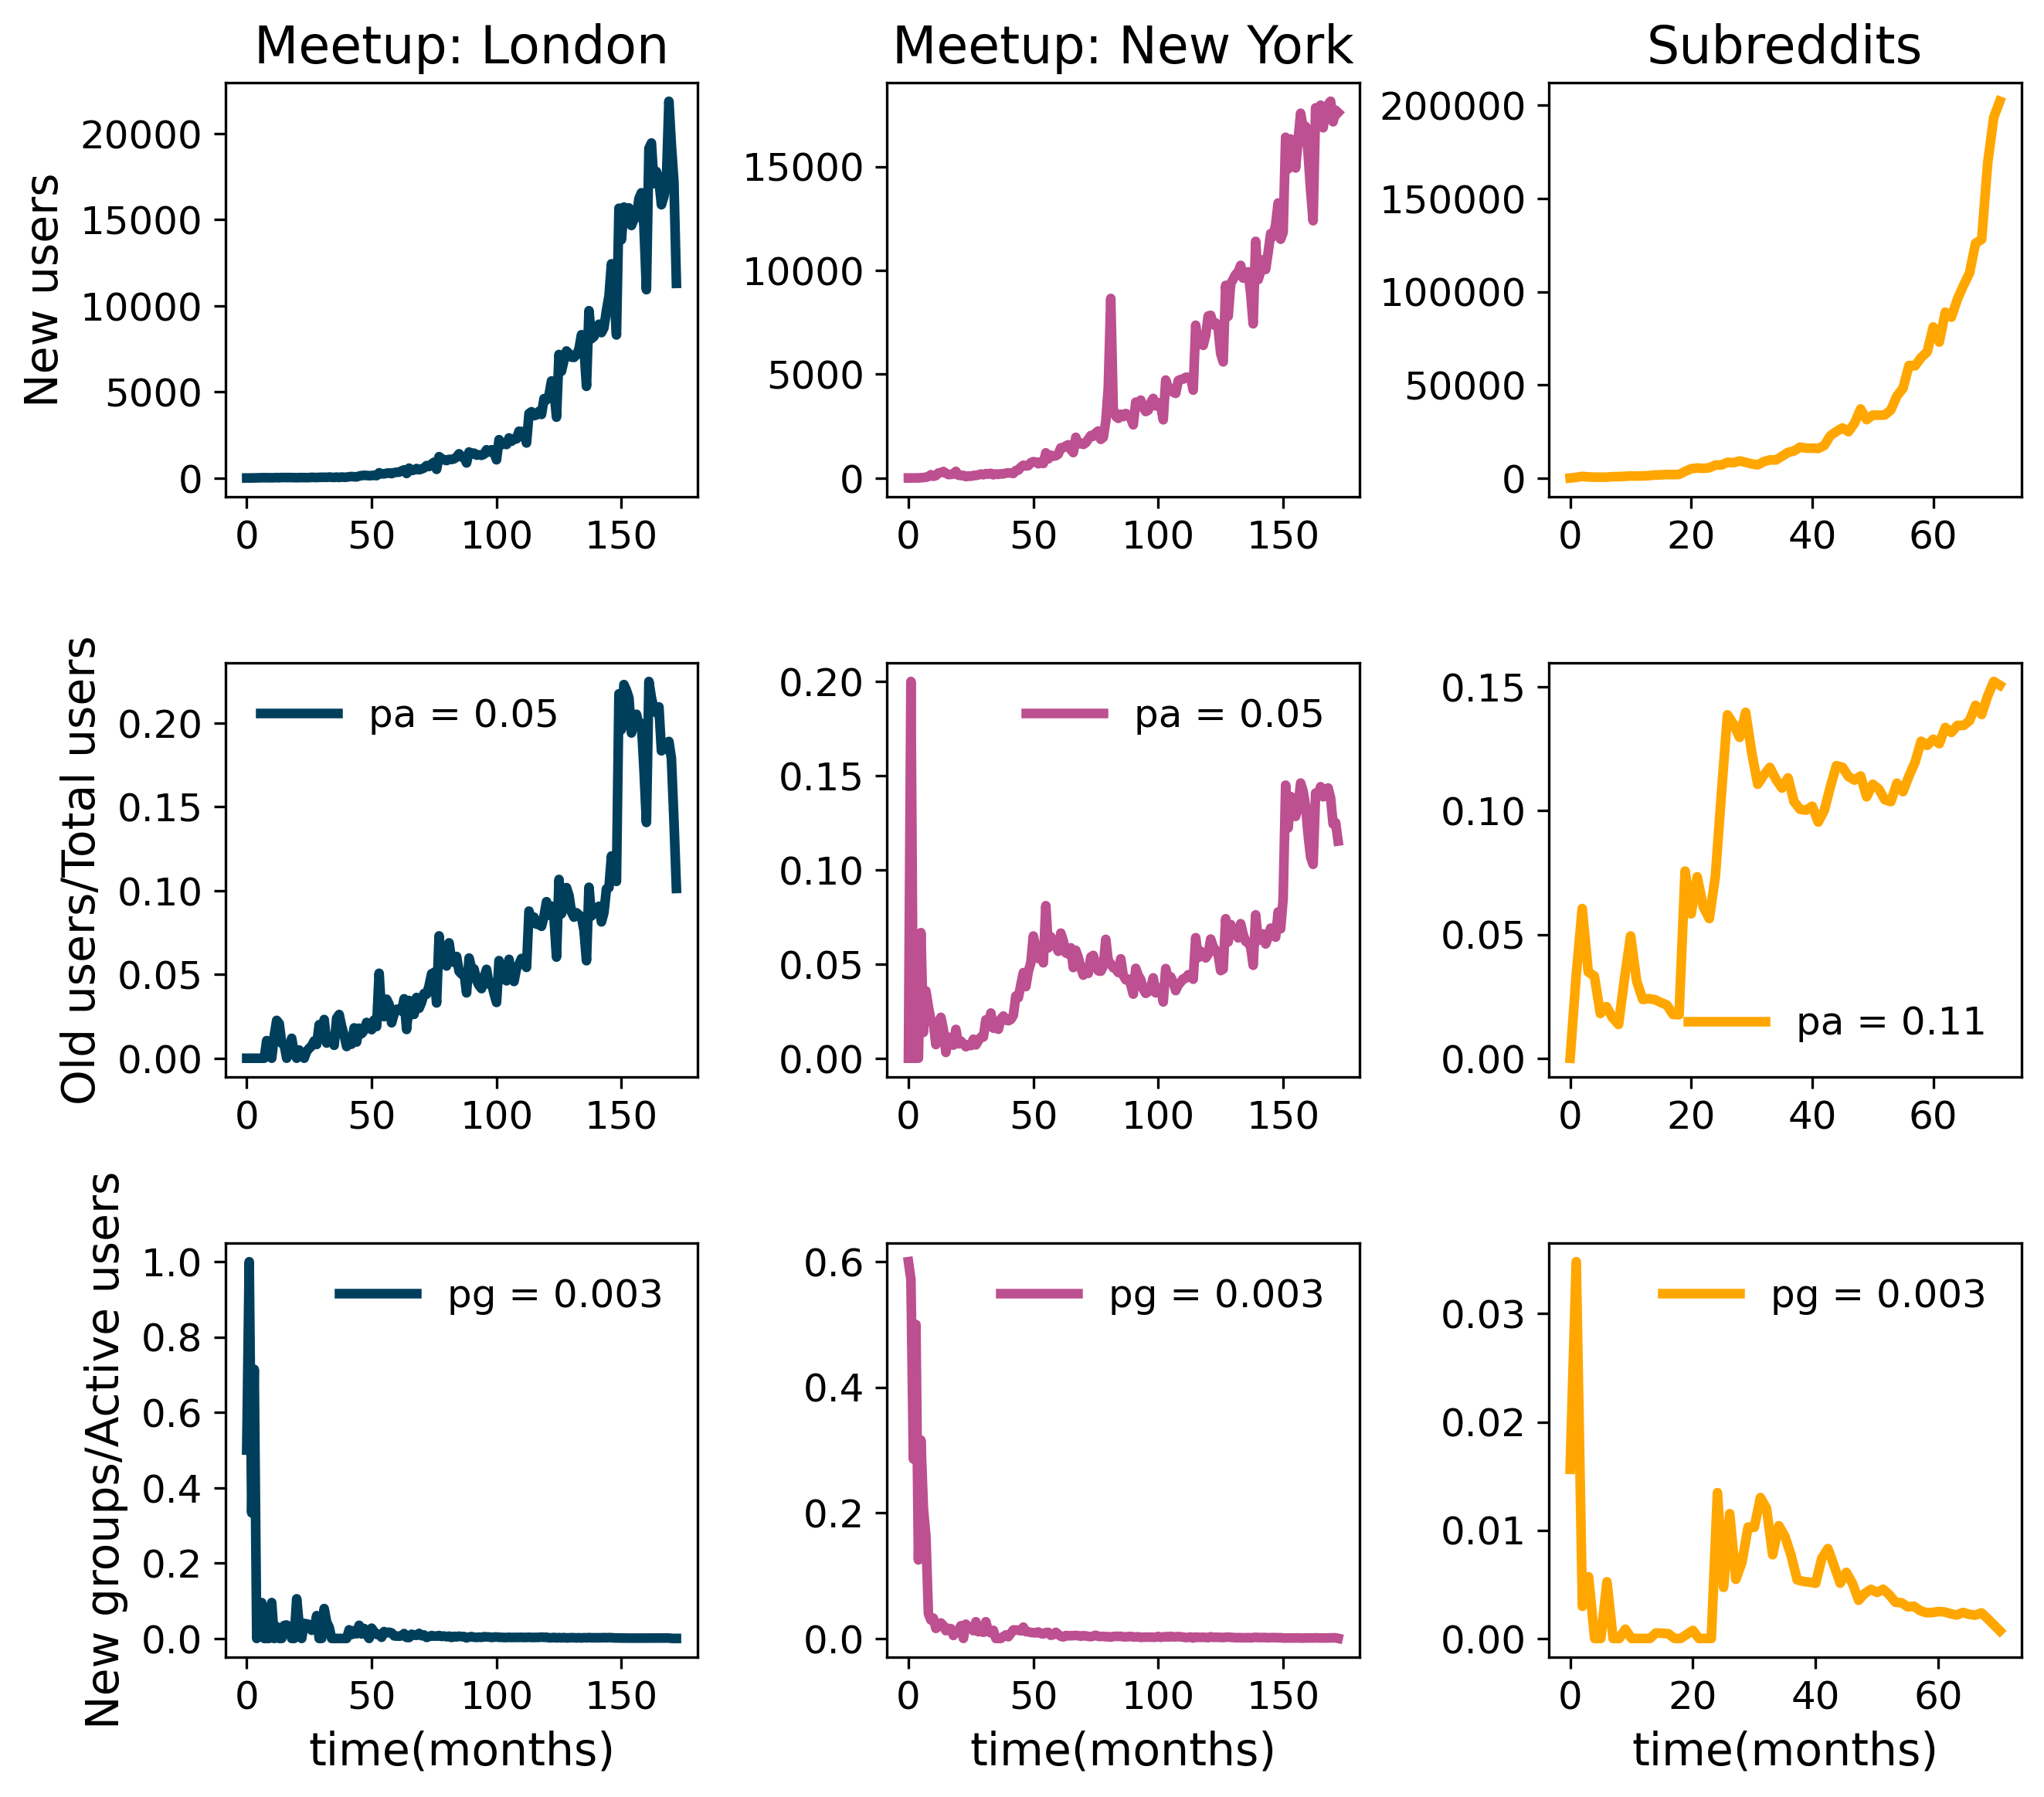
\includegraphics[width=0.8\linewidth]{Figures/figures/Fig3.png}
	\caption[The estimation of the model parameters for groups growth model.]{The time series of number of new members (top panel), ratio between old members and total members in the system (middle panel), and ratio between new groups and active members(bottom panel) for Meetup groups in London,  Meetup groups in New York, and subreddits. }
	\label{fig:fig5}
\end{figure}

The affiliation parameter $p_{aff}$ is not possible to estimate directly from the empirical data. For these reasons, we simulate the growth of social groups each of the three systems with the time series of new members obtained from the real data and estimated values of parameters $p_a$ and $p_g$, while we vary the value of $p_{aff}$. For each of the three systems, we compare the distribution of group sizes obtained from simulations for different values of $p_{aff}$ with ones obtained from empirical analysis using Jensen Shannon (JS) divergence. The JS divergence \cite{jsdivergence} between two distributions $P$ and $Q$ is defined as 
\begin{equation}
JS(P, Q) = H\left(\frac{P+Q}{2}\right) - \frac{1}{2}\left(H(P)+H(Q)\right) \label{eq2}
\end{equation}
where $H(p)$ is Shannon entropy $H(p)=\sum_x p(x)log(p(x)$. The JS divergence is symmetric and if $P$ is identical to $Q$, $JS=0$. The smaller the value of JS divergence, the better is the match between empirical and simulated group size distributions. The Table \ref{tab:table} shows the value of JS divergence for all three systems. We see that for London based Meetup groups the affiliation parameter is $p_{aff}=0.5$, for New York groups $p_{aff}=0.4$, while the affiliation parameter for Reddit $p_{aff}=0.8$. Our results show that social diffusion is important in all three systems. However, Meetup members are more likely to join groups at random, while for the Reddit members their social connections are more important when it comes to choice of the subreddit.  


\begin{table}[h]
	\centering
	\begin{tabular}{|c|c|c|c|}
		\hline
		$p_{aff}$ & JS cityLondon   & JS cityNY       & JS reddit2012    \\ \hline
		0.1  & 0.0161          & 0.0097          & 0.00241          \\ \hline
		0.2  & 0.0101          & 0.0053          & 0.00205          \\ \hline
		0.3  & 0.0055          & 0.0026          & 0.00159          \\ \hline
		0.4  & 0.0027          & \textbf{0.0013} & 0.00104          \\ \hline
		0.5  & \textbf{0.0016} & 0.0015          & 0.00074          \\ \hline
		0.6  & 0.0031          & 0.0035          & 0.00048          \\ \hline
		0.7  & 0.0085          & 0.0081          & 0.00039          \\ \hline
		0.8  & 0.0214          & 0.0167          & \textbf{0.00034} \\ \hline
		0.9  & 0.0499          & 0.0331          & 0.00047          \\ \hline
	\end{tabular}
	\caption[Jensen Shannon divergence between group sizes distributions from model and data.]{Jensen Shannon divergence between group sizes distributions from model
		(in model we vary affiliation parameter paff) and data.}
	\label{tab:table}
\end{table}


Figure \ref{fig:fig6} shows the comparison between the empirical and simulation distribution of group sizes for three considered systems. We see that empirical distributions for Meetup groups based in London and New York are perfectly reproduced by the model and chosen values of parameters. In the case of Reddit, the distribution is very broad, and the tail of distribution is well reproduced by the model.
The bottom row of Fig. \ref{fig:fig6} shows the distribution of logarithmic values of growth rates of groups obtained from empirical and simulated data. We see that the tails of empirical distributions for all three systems are well emulated by the ones obtained from the model. However, there are deviations which are the most likely consequence of using median values of parameters $p_{a}$, $p_{g}$, and $p_{aff}$.
\begin{figure}[h!]
	\centering
	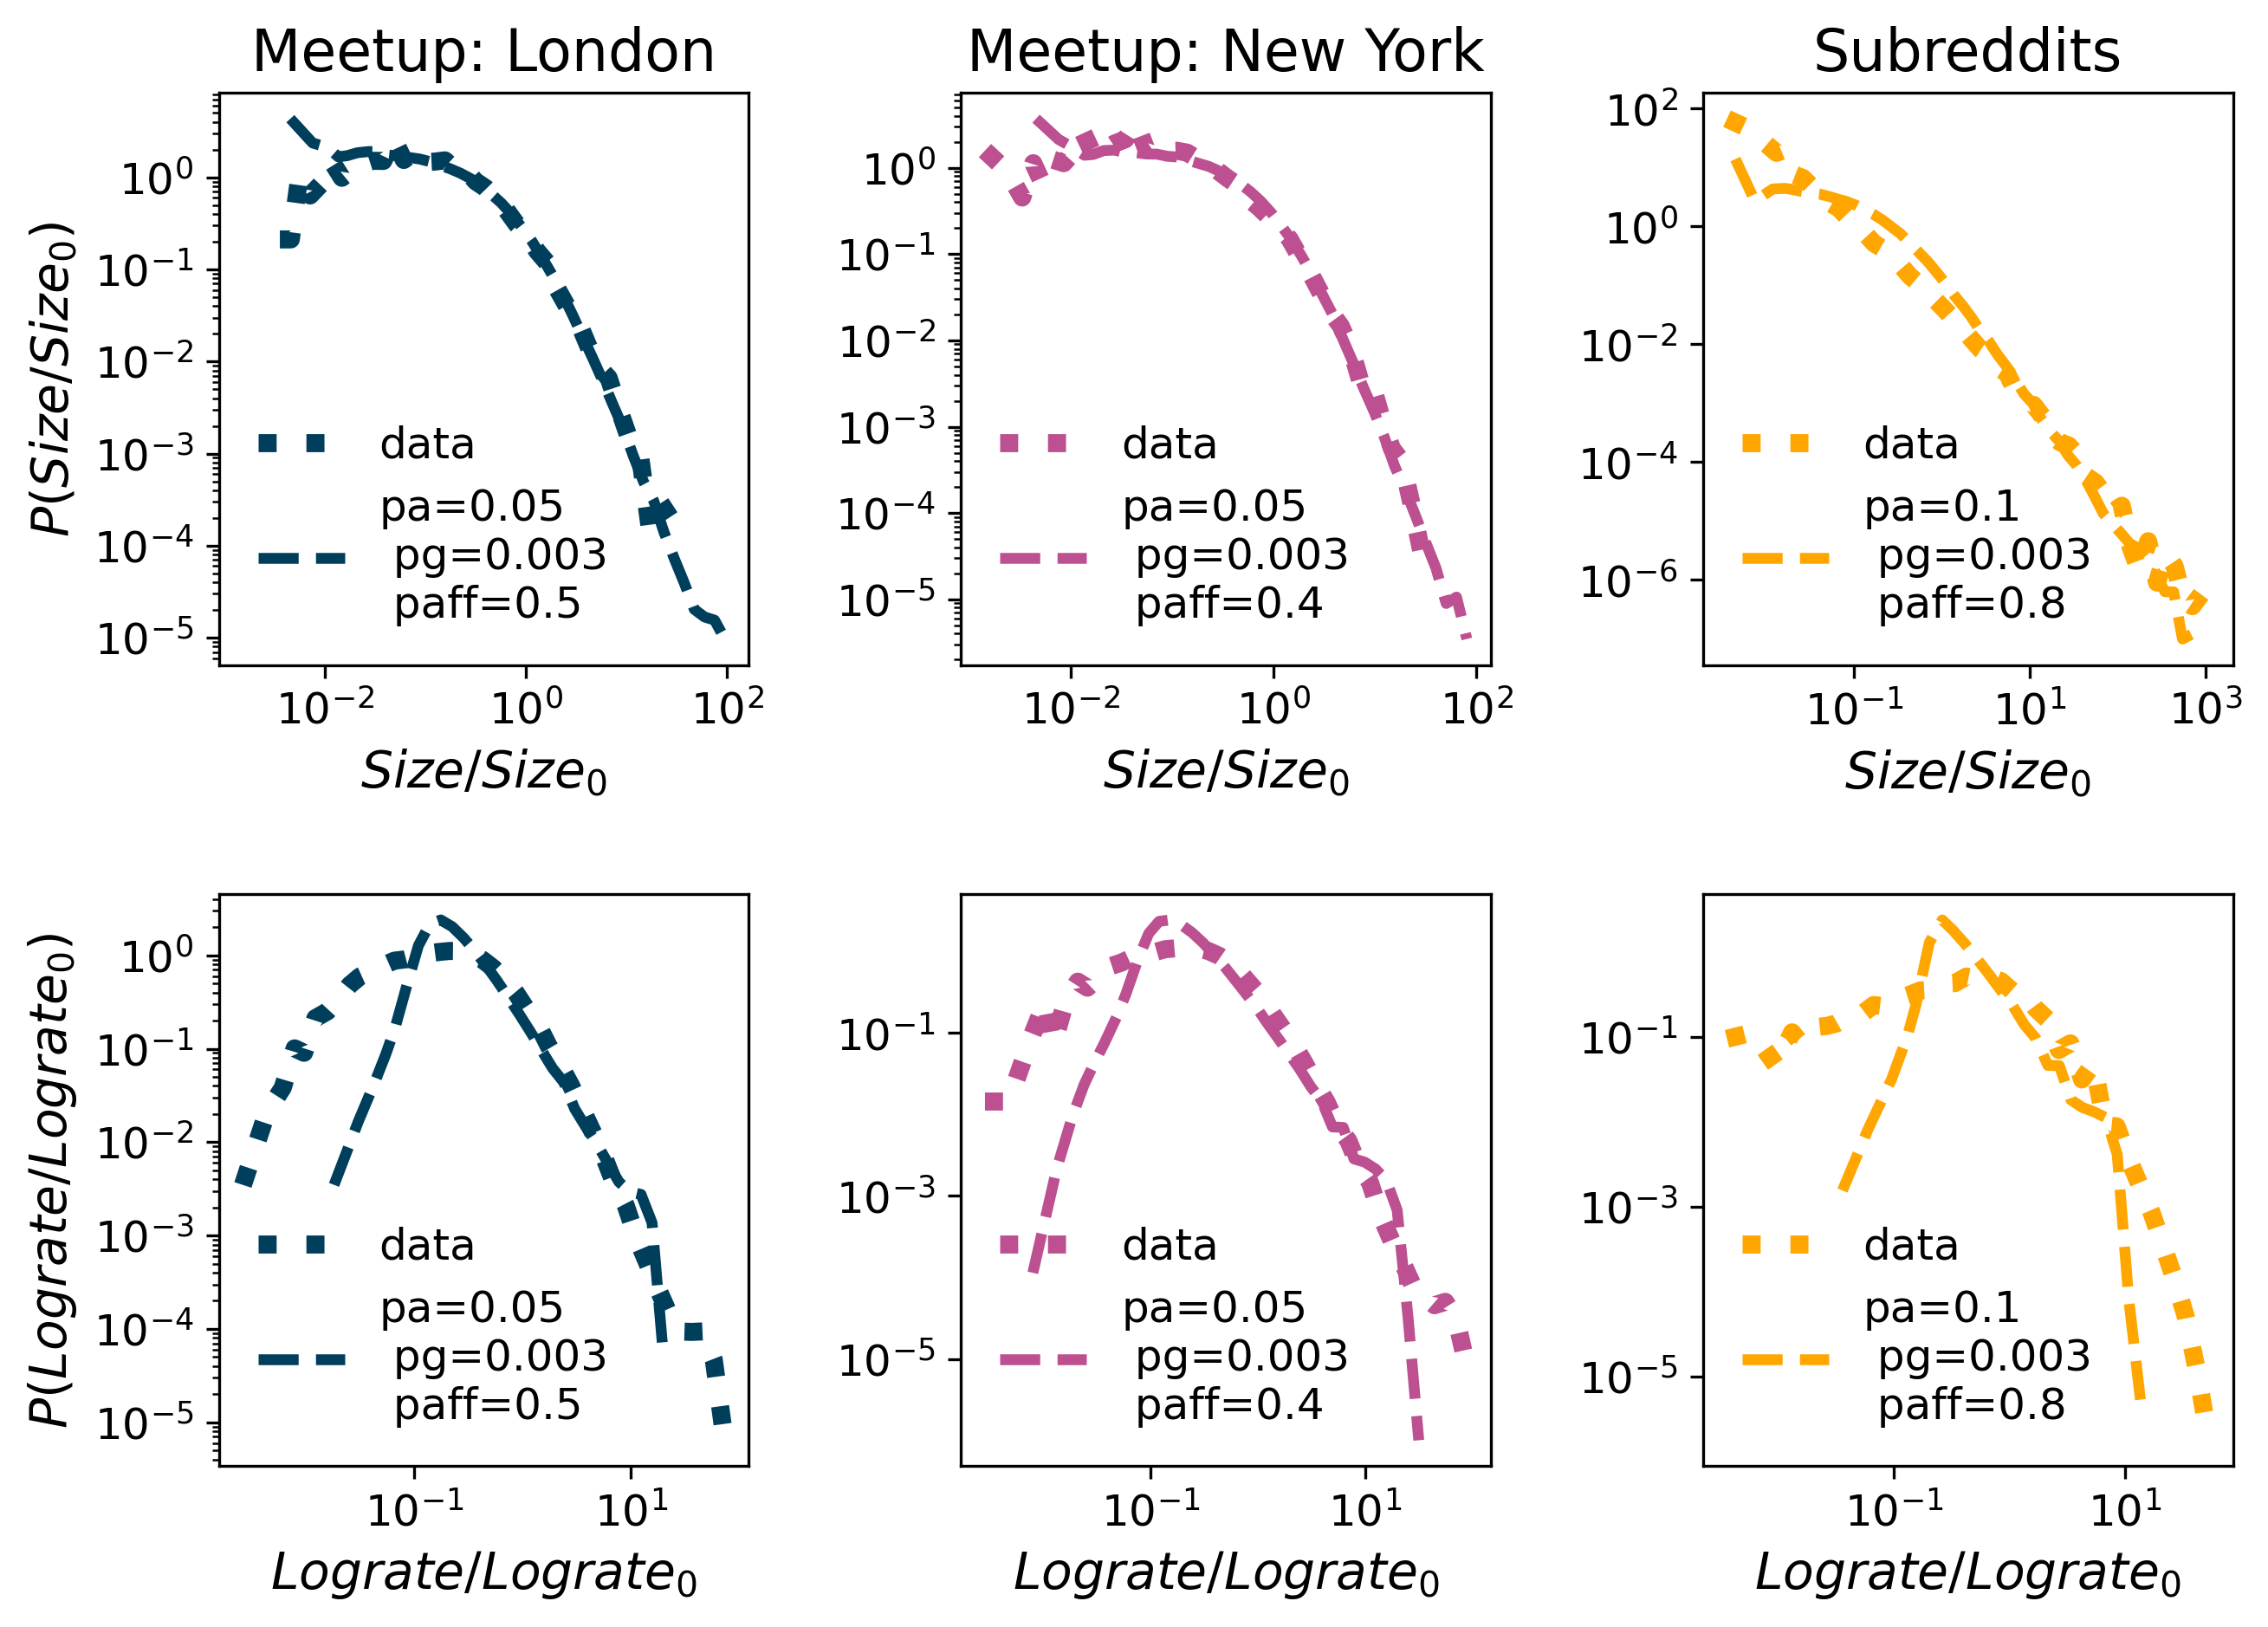
\includegraphics[width=0.8\linewidth]{Figures/figures/Fig4.png}
	\caption[The comparison between empirical and simulated data.]{The comparison between empirical and simulation distribution for group sizes (top panel) and logrates (bottom panel).}
	\label{fig:fig6}
\end{figure}

\subsection{Distributions fit}

We compute the log-likelihood ratio $R$, and $p$-value between different distributions and log-normal fit \cite{clauset2009power} to determine the best fit for the group size distributions. Distribution with a higher likelihood is a better fit. The log-likelihood ratio R then has a positive or negative value, indicating which distribution represents a better fit. To choose between two distributions, we need to calculate p-value,  to be sure that R is sufficiently positive or negative and that it is not the result of chance fluctuation from the result that is close to zero. If the p-value is small, $p<0.1$, it is unlikely that the sign of R is the chance of fluctuations, and it is an accurate indicator of which model fits better. \\

Table \ref{tab:fit-data} summarizes the findings for empirical data on group size distributions from Meetup groups in London, Meetup groups in New York and Reddit. Using the maximum likelihood method, we obtain the parameters of the distributions \cite{powerlaw}. The results indicate that log-normal distribution is the best fit for all three systems.  Figure \ref{fig:fitdata} shows the distributions of empirical data as well as log-normal fit on data. For Meetup data, we present fit on stretched exponential distribution, which very well fits a large portion of data. For subreddits, distribution is broad and, potentially, resembles power-law. Still, log-normal distribution is a more suitable fit.

\begin{table}[!ht]
	\centering
	\caption[The likelihood ratio R and p-value for fitting empirical data]{The likelihood ratio R and p-value between different candidates and \textbf{lognormal} distribution for fitting the distribution of \textbf{groups sizes} of Meetup groups in London, New York and in Reddit. According to these statistics, the lognormal distribution represents the best fit for all communities. \\ }
	\begin{tabular}{|c||cc||cc||cc|}
		\hline
		\multirow{2}{*}{\begin{tabular}[c]{@{}c@{}}distribution \end{tabular}} & \multicolumn{2}{c||}{\begin{tabular}[c]{@{}c@{}}Meetup\\ city London\end{tabular}} & \multicolumn{2}{c||}{\begin{tabular}[c]{@{}c@{}}Meetup\\ city NY\end{tabular}} & \multicolumn{2}{c|}{Reddit}                    \\ \cline{2-7} 
		& \multicolumn{1}{c|}{R}                             & p                            & \multicolumn{1}{c|}{R}                           & p                          & \multicolumn{1}{c|}{R}         & p             \\ \hline \hline \hline
		exponential                                                                            & \multicolumn{1}{c|}{-8.64e2
			%-864.86
		}                       & 8.11e-32                     & \multicolumn{1}{c|}{-8.22e2}                     & 6.63e-26                   & \multicolumn{1}{c|}{-3.85e4} & 1.54e-100     \\ \hline
		\begin{tabular}[c]{@{}c@{}}stretched \\ exponential\end{tabular}                       & \multicolumn{1}{c|}{-3.01e2}                       & 1.00e-30                      & \multicolumn{1}{c|}{-1.47e2}                     & 7.78e-8                    & \multicolumn{1}{c|}{-7.97e1}    & 5.94e-30      \\ \hline
		power law                                                                              & \multicolumn{1}{c|}{-4.88e3}                      & 0.00                         & \multicolumn{1}{c|}{-4.57e3}                    & 0.00                       & \multicolumn{1}{c|}{-9.39e2}   & 4.48e-149 \\ \hline
		\begin{tabular}[c]{@{}c@{}}truncated \\ power law\end{tabular}                         & \multicolumn{1}{c|}{-2.39e3}                      & 0.00                         & \multicolumn{1}{c|}{-2.09e3}                    & 0.00                       & \multicolumn{1}{c|}{-5.51e2}   & 2.42e-56      \\ \hline
	\end{tabular}
	\label{tab:fit-data}
\end{table}

\begin{figure}[ht]
	\centering
	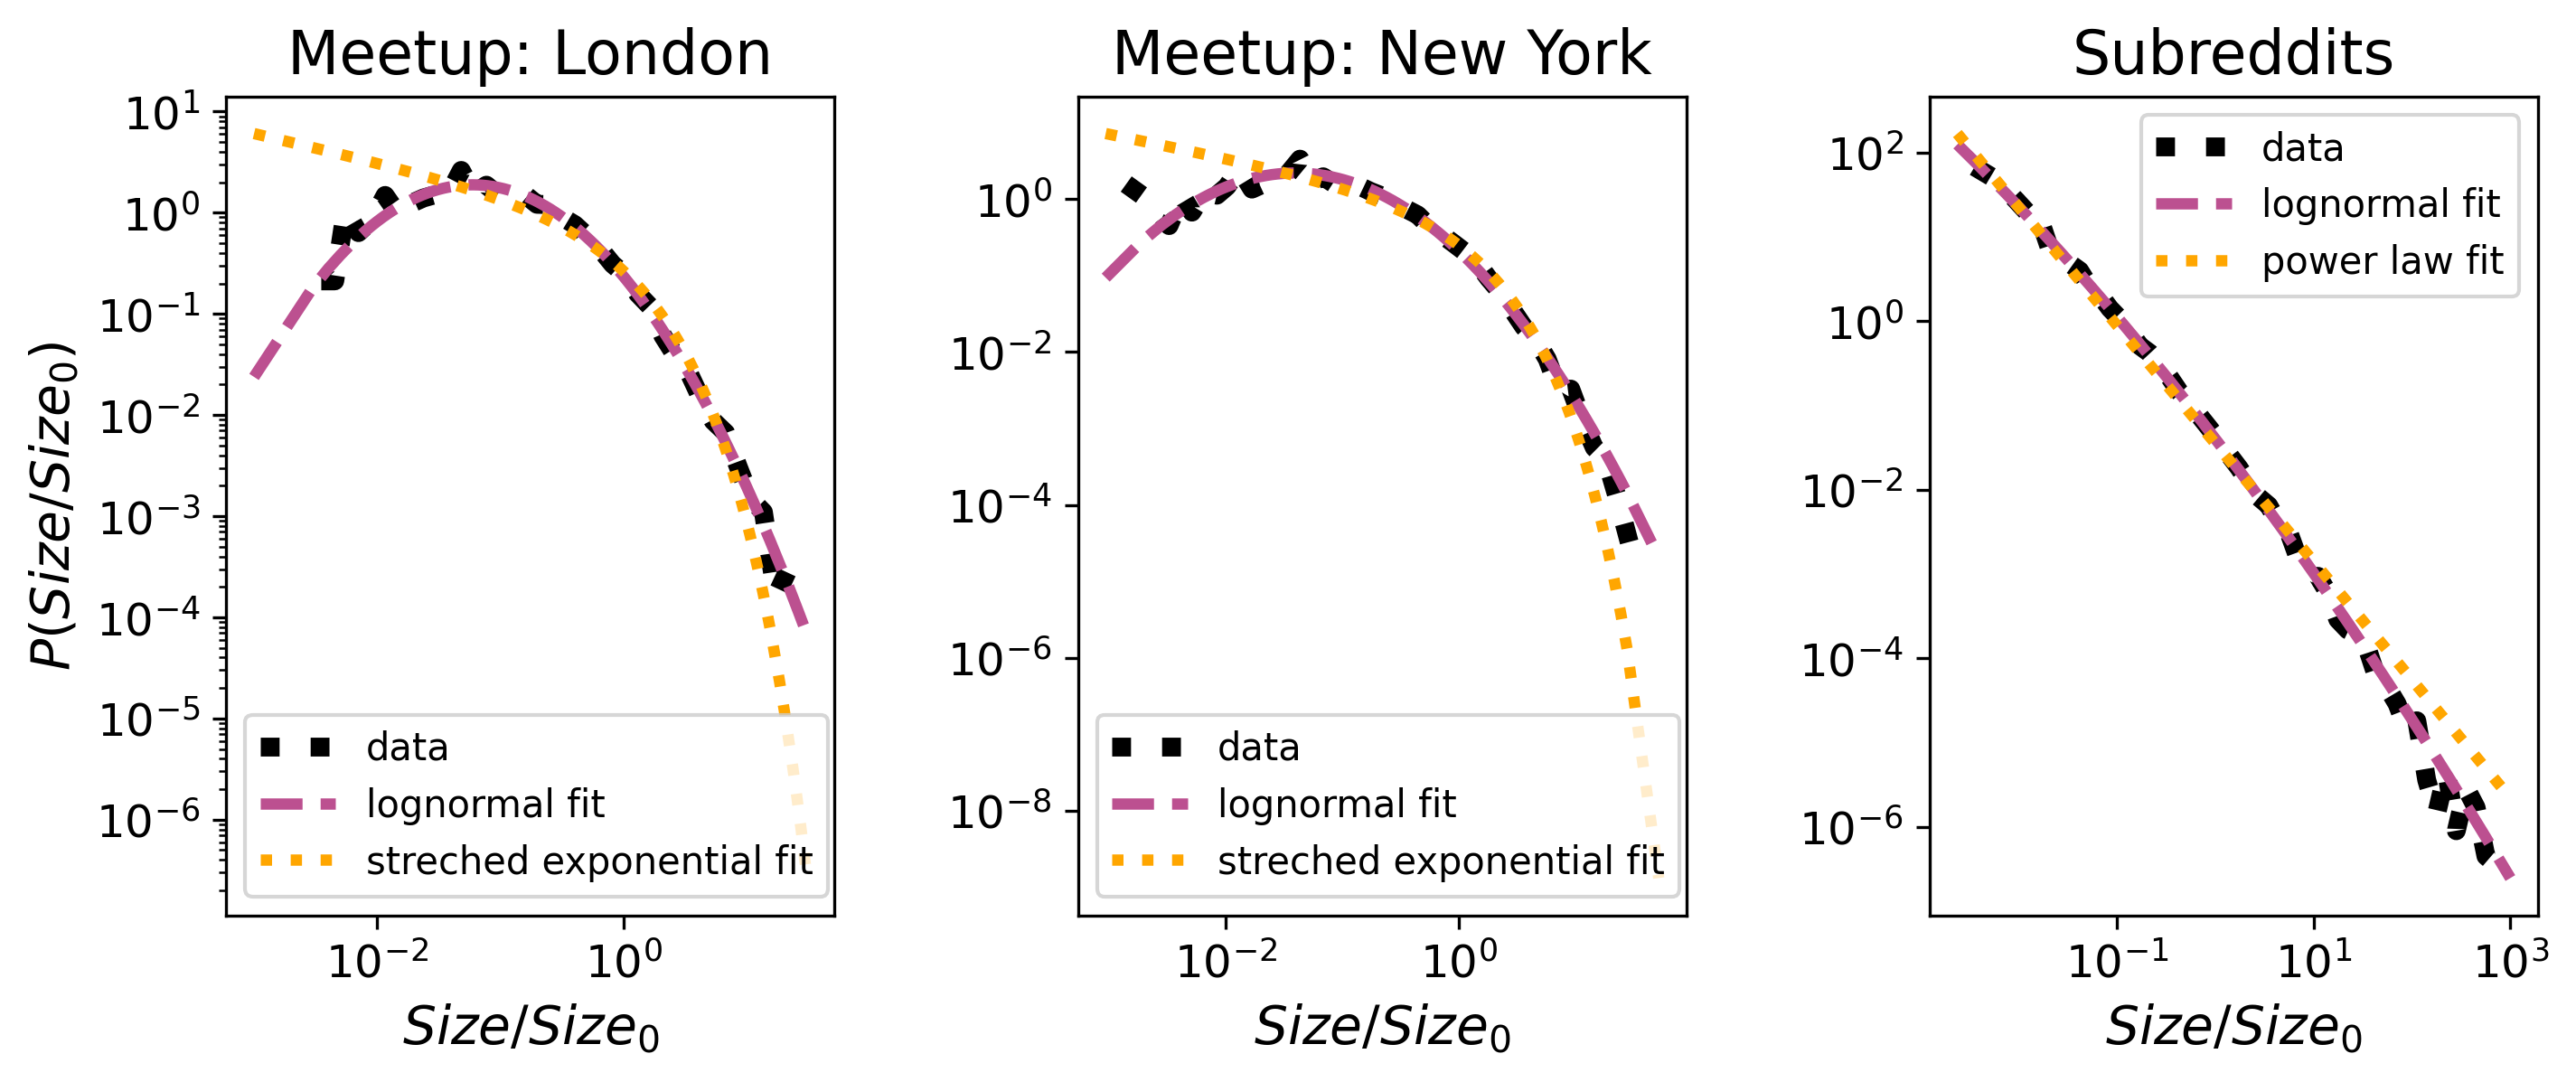
\includegraphics[width=0.8\linewidth]{figures/FigA1_data.png}
	\caption[The fitting of empirical group size distributions.]{The comparison between log-normal and stretched exponential fit to London and NY data,  and between log-normal and power law for Subreddits. The parameters for log-normal fits are 1) for city London $\mu=-0.93$ and $\sigma = 1.38$, 2) for city NY $\mu=-0.99$ and $\sigma = 1.49$, 3) for Subreddits $\mu=-5.41$ and $\sigma = 3.07$.  }
	\label{fig:fitdata}
\end{figure}

We use the same methods to estimate the fit for simulated group size distributions on Meetup groups in London, New York, and Subreddits. Table \ref{tab:fit_model} shows the results of the log-likelihood ratio R and $p$-value between different distributions. We conclude that log-normal distribution is most suitable for simulated group size distributions. Plotting log-normal and stretched exponential fit on data, Fig. \ref{fig:fit_model} we confirm our observations.  
% Please add the following required packages to your document preamble:
% \usepackage{multirow}
\begin{table}[!ht]
	\centering
	\caption[The likelihood ratio R and p-value for fitting simulated data]{The likelihood ratio R and p-value between different candidates and \textbf{lognormal}
		distribution for fitting the distribution of \textbf{simulated group sizes} of Meetup groups in London, New York and Reddit. According to these statistics, the lognormal distribution
		represents the best fit for all communities.}
	\begin{tabular}{|c||cc||cc||cc|}
		\hline
		\multirow{2}{*}{\begin{tabular}[c]{@{}c@{}}distribution \end{tabular}} & \multicolumn{2}{c||}{\begin{tabular}[c]{@{}c@{}}Meetup\\ city London\end{tabular}} & \multicolumn{2}{c||}{\begin{tabular}[c]{@{}c@{}}Meetup\\ city NY\end{tabular}} & \multicolumn{2}{c|}{Reddit}                \\ \cline{2-7} 
		& \multicolumn{1}{c|}{R}                              & p                           & \multicolumn{1}{c|}{R}                            & p                         & \multicolumn{1}{c|}{R}         & p         \\ \hline \hline \hline
		exponential                                                                            & \multicolumn{1}{c|}{-6.27e4}                      & 0.00                        & \multicolumn{1}{c|}{-5.11e4}                    & 0.00                      & \multicolumn{1}{c|}{-1.26e5} & 7.31e-125 \\ \hline
		\begin{tabular}[c]{@{}c@{}}stretched\\ exponential\end{tabular}                        & \multicolumn{1}{c|}{-1.01e4}                      & 1.96e-287                    & \multicolumn{1}{c|}{-6.69e3}                     & 1.46e-93                  & \multicolumn{1}{c|}{-1.39e4} & 0.00      \\ \hline
		power law                                                                              & \multicolumn{1}{c|}{-2.29e5}                     & 0.00                        & \multicolumn{1}{c|}{-3.73e5}                   & 0.00                      & \multicolumn{1}{c|}{-4.38e4} & 0.00      \\ \hline
		\begin{tabular}[c]{@{}c@{}}truncated\\ power law\end{tabular}                          & \multicolumn{1}{c|}{-9.28e4}                      & 0.00                        & \multicolumn{1}{c|}{-1.55e5}                   & 0.00                      & \multicolumn{1}{c|}{-9.12e4} & 0.00      \\ \hline
	\end{tabular}
	\label{tab:fit_model}
\end{table}

\clearpage
\begin{figure}[H]
	\centering
	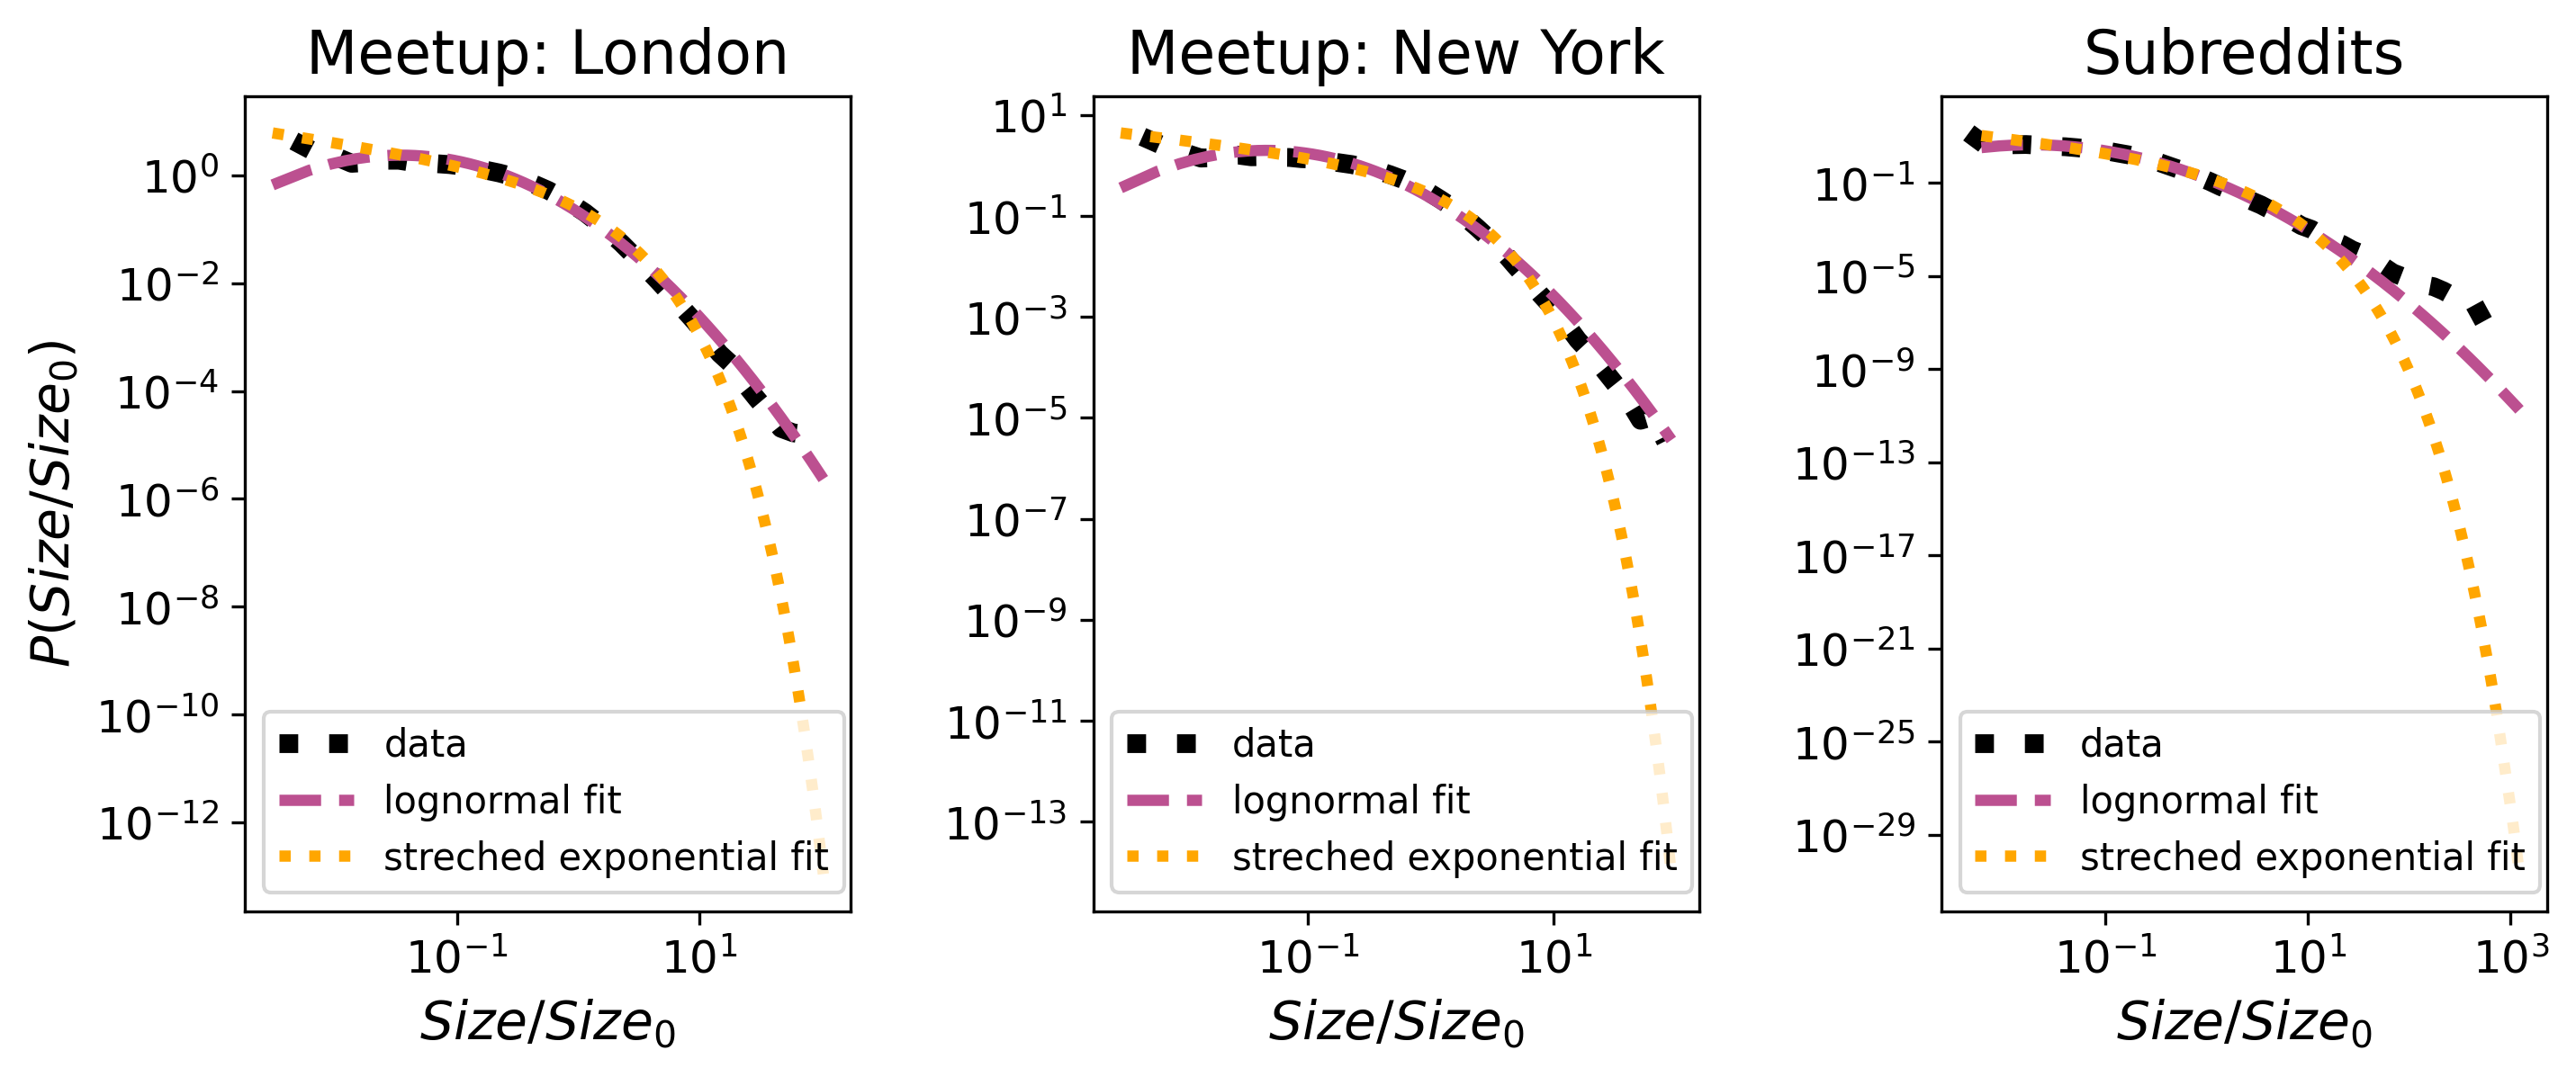
\includegraphics[width=0.8\linewidth]{figures/FigA2-model.png}
	\caption[The fitting of simulated group size distributions.]{The comparison between lognormal and stretched exponential fit to simulated group sizes distributions. The parameters for log-normal fits are 1) for city London $\mu=-0.97$ and $\sigma = 1.43$ , 2) for city NY $\mu=-0.84$ and $\sigma = 1.38$ , 3) for Subreddits $\mu=-1.63$ and $\sigma = 1.53$. }
	\label{fig:fit_model}
\end{figure}


\section{Conclusions}

We apply complex network theory and statistical physics methods to describe the evolution of online social groups, Meetups in London and NewYork and Reddits. Instead of studying user interaction networks in a single group, which is a common approach, we are interested in quantifying how users interact with the system of multiple groups and determining which processes drive the growth of groups. Similar systems have been analysed before. For example, it was found that the distribution of the cities or firms follows the log-normal and stays stable, showing universal behaviour. Contrary, the previous work on online social groups indicated that group size distributions of LiveJournal and Youtube follow power-law \cite{zheleva2009co}. On the other hand, for Meetup and Reddit we find the emergence of  log-normal distribution of groups sizes. The distribution of Reddit is much broader. Furthermore these systems grow exponentially in the number of groups and new users. 

Meetup and Reddit may be platforms with different purposes, but on the lower level, both systems could be described with the same processes users perform: they can join existing groups or create new ones. Also, in these systems, new users constantly arrive. As we find the log-normal distribution in group sizes, our first attempt was to describe this system with the Gibrat model. It is a proportional growth size model, where group size distribution converges to the log-normal distribution, while the log rates take the normal distribution. The second condition was not met, so we need to use a more intricate method.

To explore the growth of these systems in more detail, we use a model where the social system is presented with evolving bipartite and social networks \cite{zheleva2009co}. The bipartite network has partitions of users and groups, and a link exists if a user is a group member. The social network describes the social connections between members. At each time step, new users arrive in the system, following the time series of new users, and with probability, $p_a$ old members decide to be also active. The active users can create a new group with probability $p_g$; otherwise, they will join existing groups. Their decision to select a group based on social connection is determined with probability $p_{aff}$; otherwise, the choice is random. 

From empirical data we estimate model parameters $p_a$, $p_g$ and $p_{aff}$. We see that model approximates well the empirical distributions. For Meetup groups in London and New York, the $p_{aff}$ parameter is smaller, while for the Reddit $p_{aff}$ is higher, resulting in broader group sizes distribution. It also means that for Reddit members, social connections are more important for the choice of the groups. 

With results in this chapter, we contribute to the the knowledge of the growth and segmentation of the socio-economics systems. Our work was motivated by the Co-evolution model \cite{zheleva2009co}. The authors explore the social groups in which group size distribution scales as power-law. We identified different universality class, the system where group size distribution follows log normal. Further, we marked off a set of linking rules which led to log-normal group size distribution, and compared these two cases. By this, we expanded the classes of social systems that can be modelled.  


%\section{Discussion and conclusions}

%The growth of the cities and companies has attracted the attention of researchers in the previous few decades \cite{fazio2015pareto, amaral1997scaling,}. It is not surprising if we keep in mind that their growth determines other processes essential for the functioning of cities and economies. In the cities, economic and innovation growth scale with their size \cite{bettencourt2007growth}. The understanding of growth and segmentation of economic systems are essential for the long-term prediction of their evolution, and risk assessment \cite{}. The growth of social groups and social system segmentation has been slightly overlooked since the focus was mainly on the structure of social networks and their evolution.
%However, several works have studied the growth of social groups and tried to provide some insights into mechanisms that drive the growth and segmentation of social systems \cite{}.  
%The results of our empirical analysis and theoretical modeling show that there are universal growth rules that govern the growth of social groups in these systems. Through rigorous empirical analysis of the growth of social groups in three systems, Meetup groups located in London and New York, and Reddit, we show that the distribution of group sizes in these systems has log-normal normal behavior. The empirical distributions of normalized sizes of the groups created in different years fall on top of each other and have the same values of parameters for the same system. Furthermore, the distributions for Meetup groups located in London and New York have similar model parameter values, suggesting that groups' growth in these two systems are similar. Numerical simulations further confirm these findings. By tuning our model's parameters, we can reproduce the distribution of group sizes in all three systems.  

%Our results show that while the processes that govern the growth of social groups in studied social systems are the same, their importance varies among systems. The analysed groups grow through two mechanisms \cite{zheleva2009co}: members join a group that is chosen according to their interests or social relations with the group's members.

%The number of members in the system is growing, as well as the number of groups. The empirical distribution of growth rates differs for Meetup and Reddit. The observed differences can be explained by different modalities of interactions between their members. Meetup members need to invest more time and resources to interact with their peers. The events are localised in time and space, and thus the influence of peers in selecting another social group may be limited. On the other hand, Reddit members do not have these limitations. The interactions are online, asynchronous, and thus not limited in time. The influence of peers in choosing new subreddits and topics thus becomes more important. The inspection of numerical simulations confirms these observations. The values of $p_{aff}$ parameters for Meetup and Reddit imply that social connections in diffusion between groups are more critical in Reddit than in Meetup.   

%Gibrat's law is the first empirical law used by researchers to describe and explain the growth and segmentation of various socio-economical systems, including cities and firms. The possibility of application of common law to the growth of social groups in different systems indicates the existence of universal growth patterns and mechanisms that govern that growth \cite{}. Detailed and rigorous empirical analysis of the growth of the cities and firms showed that it goes beyond Gibrat's law \cite{}. Our and the work of other researchers \cite{zheleva2009co} confirm that these findings also hold for the growth of social groups. The analysis of monthly growth rates shows that these rates are log-normally distributed and depend on the size of a group. Furthermore, we cannot reduce the model proposed in this work to the law of proportional growth. Although our analysis shows that Gibrat's law does not apply to the growth of social groups, our findings confirm that universal patterns characterise this growth. 

%The results presented in this paper contribute to our knowledge of the growth and segmentation of socio-economical systems. Our rigorous analysis shows that the distribution of sizes of groups for studied systems follows a log-normal distribution. The findings of the previous research suggested the power-law behavior of this distribution. A detailed and comprehensive analysis of distributions of group sizes in social systems is needed. These and future results will help us better understand the growth and segmentation of social systems and predict their evolution and sustainability. 
%----------------------------------------------------------------------------------------


%%%%%%%%%%%%%%%%%%%%%%%%%%%%%%%%%
%Social groups, informal or formal, are mesoscopic building elements of every socio-economic system that direct its emergence, evolution, and disappearance \cite{}. The examples span from countries, economies and science to society in general. Settlements, villages, towns and cities are formal and highly structured social groups of countries. Their organisation and growth determine the functioning and sustainability of every society \cite{barthelemy2016structure}. Companies are the building blocks of an economic system and their dynamics are important indicators of the level of its development \cite{hidalgo2009building}. Scientific conferences, as scientific groups, enable fast dissemination of the latest results, exchange and evaluation of ideas as well as a knowledge extension, and thus are an integral part of science \cite{smiljanic2016theoretical}. The membership of individuals in various social groups, online and offline, can be essential when it comes to the quality of their life \cite{montazeri2001anxiety, davison2000talks, cho2012tea}. Therefore, it is not surprising that the social group emergence and evolution are at the center of the attention of many researchers \cite{aral2012identifying,gonzalez2013broadcasters, torok2013opinions, yasseri2012dynamics}.


%Along with massive data sets comes the need to develop methods and tools for their analysis and modeling. Methods and paradigms from statistical physics have proven to be very useful in studying the structure and dynamics of social systems \cite{castellano2009statistical}. The main argument for using statistical physics to study social systems is that they consist of many interacting individuals. Due to this, they exhibit different patterns in their structure and dynamics, commonly known as \textit{collective behavior}. While building units of a social systems can be characterized by many different properties, only few of them enforce collective behavior in the systems. The phenomenon is known as \textit{universality} in physics and is commonly observed in social systems such as in voting behavior \cite{chatterjee2013universality}, or scientific citations \cite{radicchi2008universality}. It indicates the existence of the universal mechanisms that govern the dynamics of the system \cite{}.


%The availability of large-scale and long-term data on various online social groups has enabled the detailed empirical study of their dynamics. The focus was mainly on the individual groups and how structural features of social interaction influence whether individuals will join the group \cite{backstrom2006group} and remain its active members \cite{smiljanic2016theoretical, smiljanic2017associative}. The study on LiveJournal \cite{backstrom2006group} groups has shown that decision of an individual to join a social group is greatly influenced by the number of her friends in the group and the structure of their interactions. The conference attendance of scientists is mainly influenced by their connections with other scientists and their sense of belonging \cite{smiljanic2016theoretical}. The sense of belonging of an individual in social groups is achieved through two main mechanisms \cite{smiljanic2017associative}: expanding of the social circle at the beginning of joining the group and strengthening of the existing connections in the later phase. The dynamics of social groups depend on their size \cite{}. Analysis of the evolution of large-scale social networks has shown that edge locality plays a critical role in the evolution of social networks \cite{leskovec2008microscopic}. Small groups are more cohesive with continued membership, while large groups tend to change their active members constantly \cite{PNAS}. These findings help us understand the growth of a single group, the evolution of its social network, and the influence of the network structure on the group growth. However, how the growth mechanisms influence the distribution of members of one social system among groups is still anecdotal.

%Furthermore, it is not clear whether the growth mechanisms of social groups are universal or system-specific. The size distribution of social groups has not been extensively studied. Rare empirical evidence of the size distribution of social groups indicates that it follows power-law behavior \cite{zheleva2009co}. However, the distribution of company sizes follows log-normal behavior and remains stable over decades \cite{amaral1997scaling, stanley1996scaling}. Analysis of the sizes of the cities shows that the distribution of all cities also follows a log-normal distribution. In contrast, the distribution of the largest cities resembles Zipf's distribution \cite{fazio2015pareto}.

%A related question that should be addressed is whether we can create a unique yet relatively simple microscopic model that reproduces the distribution of members between groups and explains the differences observed between social systems. French economist Gibrat proposed a simple growth model to reproduce the observed log-normal size distribution of companies and cities. However, the analysis of the growth rate of the companies \cite{amaral1997scaling} has shown that growth mechanisms are different from ones assumed by Gibrat. In addition, the analysis of the growth of three online social networks showed that population growth is not determined by the population size and spatial factors, and it deviates from Gibrat's law \cite{zhu2014online}. Other mechanisms, for instance, growth through diffusion, have been used for modeling and prediction of rapid group growth \cite{kairam2012life}. However, the growth mechanisms of various social groups and the source of the scaling observed in socio-economic systems remain hidden.







